\documentclass[twoside]{book}

% Packages required by doxygen
\usepackage{fixltx2e}
\usepackage{calc}
\usepackage{doxygen}
\usepackage[export]{adjustbox} % also loads graphicx
\usepackage{graphicx}
\usepackage[utf8]{inputenc}
\usepackage{makeidx}
\usepackage{multicol}
\usepackage{multirow}
\PassOptionsToPackage{warn}{textcomp}
\usepackage{textcomp}
\usepackage[nointegrals]{wasysym}
\usepackage[table]{xcolor}

% Font selection
\usepackage[T1]{fontenc}
\usepackage[scaled=.90]{helvet}
\usepackage{courier}
\usepackage{amssymb}
\usepackage{sectsty}
\renewcommand{\familydefault}{\sfdefault}
\allsectionsfont{%
  \fontseries{bc}\selectfont%
  \color{darkgray}%
}
\renewcommand{\DoxyLabelFont}{%
  \fontseries{bc}\selectfont%
  \color{darkgray}%
}
\newcommand{\+}{\discretionary{\mbox{\scriptsize$\hookleftarrow$}}{}{}}

% Page & text layout
\usepackage{geometry}
\geometry{%
  a4paper,%
  top=2.5cm,%
  bottom=2.5cm,%
  left=2.5cm,%
  right=2.5cm%
}
\tolerance=750
\hfuzz=15pt
\hbadness=750
\setlength{\emergencystretch}{15pt}
\setlength{\parindent}{0cm}
\setlength{\parskip}{3ex plus 2ex minus 2ex}
\makeatletter
\renewcommand{\paragraph}{%
  \@startsection{paragraph}{4}{0ex}{-1.0ex}{1.0ex}{%
    \normalfont\normalsize\bfseries\SS@parafont%
  }%
}
\renewcommand{\subparagraph}{%
  \@startsection{subparagraph}{5}{0ex}{-1.0ex}{1.0ex}{%
    \normalfont\normalsize\bfseries\SS@subparafont%
  }%
}
\makeatother

% Headers & footers
\usepackage{fancyhdr}
\pagestyle{fancyplain}
\fancyhead[LE]{\fancyplain{}{\bfseries\thepage}}
\fancyhead[CE]{\fancyplain{}{}}
\fancyhead[RE]{\fancyplain{}{\bfseries\leftmark}}
\fancyhead[LO]{\fancyplain{}{\bfseries\rightmark}}
\fancyhead[CO]{\fancyplain{}{}}
\fancyhead[RO]{\fancyplain{}{\bfseries\thepage}}
\fancyfoot[LE]{\fancyplain{}{}}
\fancyfoot[CE]{\fancyplain{}{}}
\fancyfoot[RE]{\fancyplain{}{\bfseries\scriptsize Generated by Doxygen }}
\fancyfoot[LO]{\fancyplain{}{\bfseries\scriptsize Generated by Doxygen }}
\fancyfoot[CO]{\fancyplain{}{}}
\fancyfoot[RO]{\fancyplain{}{}}
\renewcommand{\footrulewidth}{0.4pt}
\renewcommand{\chaptermark}[1]{%
  \markboth{#1}{}%
}
\renewcommand{\sectionmark}[1]{%
  \markright{\thesection\ #1}%
}

% Indices & bibliography
\usepackage{natbib}
\usepackage[titles]{tocloft}
\setcounter{tocdepth}{3}
\setcounter{secnumdepth}{5}
\makeindex

% Hyperlinks (required, but should be loaded last)
\usepackage{ifpdf}
\ifpdf
  \usepackage[pdftex,pagebackref=true]{hyperref}
\else
  \usepackage[ps2pdf,pagebackref=true]{hyperref}
\fi
\hypersetup{%
  colorlinks=true,%
  linkcolor=blue,%
  citecolor=blue,%
  unicode%
}

% Custom commands
\newcommand{\clearemptydoublepage}{%
  \newpage{\pagestyle{empty}\cleardoublepage}%
}

\usepackage{caption}
\captionsetup{labelsep=space,justification=centering,font={bf},singlelinecheck=off,skip=4pt,position=top}

%===== C O N T E N T S =====

\begin{document}

% Titlepage & ToC
\hypersetup{pageanchor=false,
             bookmarksnumbered=true,
             pdfencoding=unicode
            }
\pagenumbering{alph}
\begin{titlepage}
\vspace*{7cm}
\begin{center}%
{\Large Trajetoria\+Direcional }\\
\vspace*{1cm}
{\large Generated by Doxygen 1.8.13}\\
\end{center}
\end{titlepage}
\clearemptydoublepage
\pagenumbering{roman}
\tableofcontents
\clearemptydoublepage
\pagenumbering{arabic}
\hypersetup{pageanchor=true}

%--- Begin generated contents ---
\chapter{Class Index}
\section{Class List}
Here are the classes, structs, unions and interfaces with brief descriptions\+:\begin{DoxyCompactList}
\item\contentsline{section}{\hyperlink{class_c_parametros_direcional}{C\+Parametros\+Direcional} }{\pageref{class_c_parametros_direcional}}{}
\item\contentsline{section}{\hyperlink{class_c_simulador}{C\+Simulador} \\*O S\+I\+M\+U\+L\+A\+D\+OR R\+E\+U\+N\+IE T\+O\+D\+AS AS C\+L\+A\+S\+S\+ES E A\+C\+E\+S\+SA T\+O\+D\+AS P\+A\+RA C\+H\+A\+M\+AR OS R\+E\+S\+U\+L\+T\+A\+D\+OS }{\pageref{class_c_simulador}}{}
\item\contentsline{section}{\hyperlink{class_c_traj_direcional}{C\+Traj\+Direcional} \\*P\+A\+RA I\+S\+SO P\+R\+E\+C\+I\+S\+A\+M\+OS I\+N\+C\+L\+U\+IR T\+O\+D\+AS AS C\+L\+A\+S\+S\+ES }{\pageref{class_c_traj_direcional}}{}
\item\contentsline{section}{\hyperlink{class_c_traj_direcional_build_up}{C\+Traj\+Direcional\+Build\+Up} \\*U\+T\+I\+L\+I\+Z\+AR OS P\+A\+RÂ\+M\+E\+T\+R\+OS D\+I\+R\+E\+C\+I\+O\+N\+A\+IS C\+A\+L\+C\+U\+L\+A\+D\+OS NA C\+L\+A\+S\+SE \char`\"{}\+C\+P\+A\+R\+A\+M\+E\+T\+R\+O\+S\+D\+I\+R\+E\+C\+I\+O\+N\+A\+L\char`\"{} }{\pageref{class_c_traj_direcional_build_up}}{}
\item\contentsline{section}{\hyperlink{class_c_traj_direcional_slant}{C\+Traj\+Direcional\+Slant} }{\pageref{class_c_traj_direcional_slant}}{}
\item\contentsline{section}{\hyperlink{class_c_traj_vertical}{C\+Traj\+Vertical} }{\pageref{class_c_traj_vertical}}{}
\end{DoxyCompactList}

\chapter{Class Documentation}
\hypertarget{class_c_parametros_direcional}{}\section{C\+Parametros\+Direcional Class Reference}
\label{class_c_parametros_direcional}\index{C\+Parametros\+Direcional@{C\+Parametros\+Direcional}}


Collaboration diagram for C\+Parametros\+Direcional\+:
\nopagebreak
\begin{figure}[H]
\begin{center}
\leavevmode
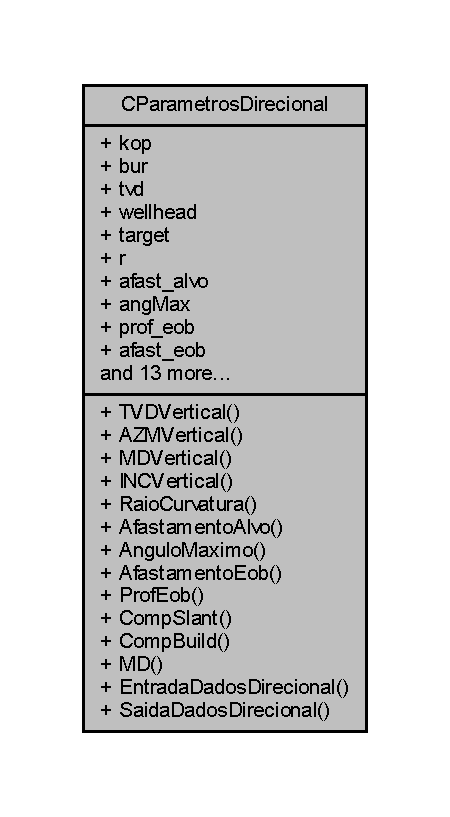
\includegraphics[width=216pt]{class_c_parametros_direcional__coll__graph}
\end{center}
\end{figure}
\subsection*{Public Member Functions}
\begin{DoxyCompactItemize}
\item 
void \hyperlink{class_c_parametros_direcional_abdebc36ad859b6e46129ffa0a5a90bc9}{T\+V\+D\+Vertical} ()
\item 
void \hyperlink{class_c_parametros_direcional_afbc3332ccc36d3cabafae5cc7e90bfdb}{A\+Z\+M\+Vertical} ()
\begin{DoxyCompactList}\small\item\em M�\+T\+O\+D\+OS V\+E\+R\+T\+I\+C\+A\+IS. \end{DoxyCompactList}\item 
void \hyperlink{class_c_parametros_direcional_a683aced24a9b0d2dda361435ff973558}{M\+D\+Vertical} ()
\item 
void \hyperlink{class_c_parametros_direcional_a4279fb5351003e8b4e492583fe90c47b}{I\+N\+C\+Vertical} ()
\item 
void \hyperlink{class_c_parametros_direcional_a427ce1e4434a193d8741edfd39ad3556}{Raio\+Curvatura} ()
\item 
void \hyperlink{class_c_parametros_direcional_a89123fe01dacfe6c3980ba4285af7e90}{Afastamento\+Alvo} ()
\begin{DoxyCompactList}\small\item\em M�\+T\+O\+D\+OS DA C\+L\+A\+S\+SE Q\+UE C\+A\+L\+C\+U\+L\+AM OS P\+A\+R�\+M\+E\+T\+R\+OS D\+I\+R\+E\+C\+I\+O\+N\+A\+IS U\+T\+I\+L\+I\+Z\+A\+D\+OS N\+AS T\+R\+A\+J\+E\+T�\+R\+I\+AS. \end{DoxyCompactList}\item 
void \hyperlink{class_c_parametros_direcional_a14c6c5d28c1f19390bfdb9ca705373d7}{Angulo\+Maximo} ()
\item 
void \hyperlink{class_c_parametros_direcional_a986fb23a4f4e615eeefaf23050dd1a54}{Afastamento\+Eob} ()
\item 
void \hyperlink{class_c_parametros_direcional_ae69da1afeb29517aa0cd87e96020ea29}{Prof\+Eob} ()
\item 
void \hyperlink{class_c_parametros_direcional_a58f99af659ac211d50027f7e2feb0c39}{Comp\+Slant} ()
\item 
void \hyperlink{class_c_parametros_direcional_adfa8d6781c2c43c69cf64b558fb55874}{Comp\+Build} ()
\item 
void \hyperlink{class_c_parametros_direcional_a323a405039a4c5a4248999f7a4f0e8b6}{MD} ()
\item 
void \hyperlink{class_c_parametros_direcional_a6ed5f69e3761f1213c03ffcccf699800}{Entrada\+Dados\+Direcional} ()
\item 
void \hyperlink{class_c_parametros_direcional_acee86bd5906c882c287505319c3ed1bb}{Saida\+Dados\+Direcional} ()
\begin{DoxyCompactList}\small\item\em M�\+T\+O\+DO R\+E\+C\+E\+BE T\+O\+D\+OS OS D\+A\+D\+OS. \end{DoxyCompactList}\end{DoxyCompactItemize}
\subsection*{Public Attributes}
\begin{DoxyCompactItemize}
\item 
\mbox{\Hypertarget{class_c_parametros_direcional_a1c19d71599fb0407592b340f239b5453}\label{class_c_parametros_direcional_a1c19d71599fb0407592b340f239b5453}} 
double {\bfseries kop}
\item 
\mbox{\Hypertarget{class_c_parametros_direcional_a701682b83486a306bf95aad1299a5e85}\label{class_c_parametros_direcional_a701682b83486a306bf95aad1299a5e85}} 
double \hyperlink{class_c_parametros_direcional_a701682b83486a306bf95aad1299a5e85}{bur}
\begin{DoxyCompactList}\small\item\em D\+E\+C\+L\+A\+R\+A��O DE T\+O\+D\+OS OS A\+T\+R\+I\+B\+U\+T\+OS Q\+UE S\+E\+R�O U\+T\+I\+L\+I\+Z\+A\+D\+OS. \end{DoxyCompactList}\item 
\mbox{\Hypertarget{class_c_parametros_direcional_a7f703826cd3f2b5761de1e582ff1c344}\label{class_c_parametros_direcional_a7f703826cd3f2b5761de1e582ff1c344}} 
double {\bfseries tvd}
\item 
\mbox{\Hypertarget{class_c_parametros_direcional_ad0e117e5e1d4437effc4cd8f296939d4}\label{class_c_parametros_direcional_ad0e117e5e1d4437effc4cd8f296939d4}} 
double {\bfseries wellhead} \mbox{[}2\mbox{]}
\item 
\mbox{\Hypertarget{class_c_parametros_direcional_a49eb9e4f5851ab56ff01b5f55617a589}\label{class_c_parametros_direcional_a49eb9e4f5851ab56ff01b5f55617a589}} 
double {\bfseries target} \mbox{[}2\mbox{]}
\item 
\mbox{\Hypertarget{class_c_parametros_direcional_a848e52c50ba96e69153b337edd65c673}\label{class_c_parametros_direcional_a848e52c50ba96e69153b337edd65c673}} 
double {\bfseries r}
\item 
\mbox{\Hypertarget{class_c_parametros_direcional_a76badc22870158d3ded64d2438b46df2}\label{class_c_parametros_direcional_a76badc22870158d3ded64d2438b46df2}} 
double {\bfseries afast\+\_\+alvo}
\item 
\mbox{\Hypertarget{class_c_parametros_direcional_a17906cb631dd54fa2b2bde4b8e063d67}\label{class_c_parametros_direcional_a17906cb631dd54fa2b2bde4b8e063d67}} 
double {\bfseries ang\+Max}
\item 
\mbox{\Hypertarget{class_c_parametros_direcional_a3d970648c437e14d0d1cd0ae84da9205}\label{class_c_parametros_direcional_a3d970648c437e14d0d1cd0ae84da9205}} 
double {\bfseries prof\+\_\+eob}
\item 
\mbox{\Hypertarget{class_c_parametros_direcional_a7b41a3196dce5ac3ae251b7246538ade}\label{class_c_parametros_direcional_a7b41a3196dce5ac3ae251b7246538ade}} 
double {\bfseries afast\+\_\+eob}
\item 
\mbox{\Hypertarget{class_c_parametros_direcional_ab5e961d4ba2cfe2b7518cde5ddadb022}\label{class_c_parametros_direcional_ab5e961d4ba2cfe2b7518cde5ddadb022}} 
double {\bfseries comp\+\_\+build}
\item 
\mbox{\Hypertarget{class_c_parametros_direcional_ad666ab5139b3ec6ce9c6f8bc426658c0}\label{class_c_parametros_direcional_ad666ab5139b3ec6ce9c6f8bc426658c0}} 
double {\bfseries comp\+\_\+slant}
\item 
\mbox{\Hypertarget{class_c_parametros_direcional_a58d13de700bd4d007acef635ada1b936}\label{class_c_parametros_direcional_a58d13de700bd4d007acef635ada1b936}} 
double {\bfseries K}
\item 
\mbox{\Hypertarget{class_c_parametros_direcional_a0a507137afdf3791eaf47ba77f8e29fb}\label{class_c_parametros_direcional_a0a507137afdf3791eaf47ba77f8e29fb}} 
double {\bfseries md\+\_\+total}
\item 
double \hyperlink{class_c_parametros_direcional_aa9d61e2c4488fdcf263de66aebad5c96}{azm}
\item 
\mbox{\Hypertarget{class_c_parametros_direcional_a196ac0ef4285e8f2a1d383d68dfcb84f}\label{class_c_parametros_direcional_a196ac0ef4285e8f2a1d383d68dfcb84f}} 
double \hyperlink{class_c_parametros_direcional_a196ac0ef4285e8f2a1d383d68dfcb84f}{A}
\begin{DoxyCompactList}\small\item\em P\+A\+R�\+M\+E\+T\+R\+OS U\+T\+I\+L\+I\+Z\+A\+D\+OS N\+OS C�\+L\+C\+U\+L\+OS DA S\+E��O V\+E\+R\+T\+I\+C\+AL. \end{DoxyCompactList}\item 
\mbox{\Hypertarget{class_c_parametros_direcional_aaa0909dc588941d379d8671d694c9a01}\label{class_c_parametros_direcional_aaa0909dc588941d379d8671d694c9a01}} 
double {\bfseries B}
\item 
\mbox{\Hypertarget{class_c_parametros_direcional_a460ac771873d419b4cb0e396ba618d02}\label{class_c_parametros_direcional_a460ac771873d419b4cb0e396ba618d02}} 
double {\bfseries C}
\item 
\mbox{\Hypertarget{class_c_parametros_direcional_afaff2d4e6ebc54bf46b17ed9fe67c963}\label{class_c_parametros_direcional_afaff2d4e6ebc54bf46b17ed9fe67c963}} 
int {\bfseries tamanho}
\item 
\mbox{\Hypertarget{class_c_parametros_direcional_a953ae514e88495fe746c3d2086ab621e}\label{class_c_parametros_direcional_a953ae514e88495fe746c3d2086ab621e}} 
std\+::vector$<$ double $>$ {\bfseries tvd\+Vertical}
\item 
\mbox{\Hypertarget{class_c_parametros_direcional_a2bf1d7aa5e6172a63fe7ea2c4acd4127}\label{class_c_parametros_direcional_a2bf1d7aa5e6172a63fe7ea2c4acd4127}} 
std\+::vector$<$ double $>$ \hyperlink{class_c_parametros_direcional_a2bf1d7aa5e6172a63fe7ea2c4acd4127}{azimute}
\begin{DoxyCompactList}\small\item\em V\+E\+T\+O\+R\+ES V\+E\+R\+T\+I\+C\+A\+IS. \end{DoxyCompactList}\item 
\mbox{\Hypertarget{class_c_parametros_direcional_aa189f841c6f9faf3bcdc8ef8afe6291b}\label{class_c_parametros_direcional_aa189f841c6f9faf3bcdc8ef8afe6291b}} 
std\+::vector$<$ double $>$ {\bfseries md\+Vertical}
\item 
\mbox{\Hypertarget{class_c_parametros_direcional_a3175f3f60bfae71f072061a1a6921a1d}\label{class_c_parametros_direcional_a3175f3f60bfae71f072061a1a6921a1d}} 
std\+::vector$<$ double $>$ {\bfseries inc\+Vertical}
\end{DoxyCompactItemize}


\subsection{Member Function Documentation}
\mbox{\Hypertarget{class_c_parametros_direcional_a89123fe01dacfe6c3980ba4285af7e90}\label{class_c_parametros_direcional_a89123fe01dacfe6c3980ba4285af7e90}} 
\index{C\+Parametros\+Direcional@{C\+Parametros\+Direcional}!Afastamento\+Alvo@{Afastamento\+Alvo}}
\index{Afastamento\+Alvo@{Afastamento\+Alvo}!C\+Parametros\+Direcional@{C\+Parametros\+Direcional}}
\subsubsection{\texorpdfstring{Afastamento\+Alvo()}{AfastamentoAlvo()}}
{\footnotesize\ttfamily void C\+Parametros\+Direcional\+::\+Afastamento\+Alvo (\begin{DoxyParamCaption}{ }\end{DoxyParamCaption})}



M�\+T\+O\+D\+OS DA C\+L\+A\+S\+SE Q\+UE C\+A\+L\+C\+U\+L\+AM OS P\+A\+R�\+M\+E\+T\+R\+OS D\+I\+R\+E\+C\+I\+O\+N\+A\+IS U\+T\+I\+L\+I\+Z\+A\+D\+OS N\+AS T\+R\+A\+J\+E\+T�\+R\+I\+AS. 

O A\+F\+A\+S\+T\+A\+M\+E\+N\+TO � C\+A\+L\+C\+U\+L\+A\+DO A P\+A\+R\+T\+IR D\+AS C\+O\+O\+R\+D\+E\+N\+A\+D\+AS DA S\+O\+N\+DA E DO A\+L\+VO \mbox{\Hypertarget{class_c_parametros_direcional_a986fb23a4f4e615eeefaf23050dd1a54}\label{class_c_parametros_direcional_a986fb23a4f4e615eeefaf23050dd1a54}} 
\index{C\+Parametros\+Direcional@{C\+Parametros\+Direcional}!Afastamento\+Eob@{Afastamento\+Eob}}
\index{Afastamento\+Eob@{Afastamento\+Eob}!C\+Parametros\+Direcional@{C\+Parametros\+Direcional}}
\subsubsection{\texorpdfstring{Afastamento\+Eob()}{AfastamentoEob()}}
{\footnotesize\ttfamily void C\+Parametros\+Direcional\+::\+Afastamento\+Eob (\begin{DoxyParamCaption}{ }\end{DoxyParamCaption})}

E\+S\+TE M�\+T\+O\+DO C\+A\+L\+C\+U\+LA O A\+F\+A\+S\+T\+A\+M\+E\+N\+TO H\+O\+R\+I\+Z\+O\+N\+T\+AL NO F\+I\+N\+AL DA S\+E��O DE G\+A\+N\+HO DE �\+N\+G\+U\+LO \mbox{\Hypertarget{class_c_parametros_direcional_a14c6c5d28c1f19390bfdb9ca705373d7}\label{class_c_parametros_direcional_a14c6c5d28c1f19390bfdb9ca705373d7}} 
\index{C\+Parametros\+Direcional@{C\+Parametros\+Direcional}!Angulo\+Maximo@{Angulo\+Maximo}}
\index{Angulo\+Maximo@{Angulo\+Maximo}!C\+Parametros\+Direcional@{C\+Parametros\+Direcional}}
\subsubsection{\texorpdfstring{Angulo\+Maximo()}{AnguloMaximo()}}
{\footnotesize\ttfamily void C\+Parametros\+Direcional\+::\+Angulo\+Maximo (\begin{DoxyParamCaption}{ }\end{DoxyParamCaption})}

O �\+N\+G\+U\+LO M�\+X\+I\+MO R\+E\+P\+R\+E\+S\+E\+N\+TA A M�\+X\+I\+MA I\+N\+C\+L\+I\+N\+A��O Q\+UE O P\+O�O I\+R� A\+L\+C\+A\+N�\+AR

V\+A\+R\+I�\+V\+E\+IS L\+O\+C\+A\+IS C\+R\+I\+A\+D\+AS P\+A\+RA F\+A\+C\+I\+L\+I\+T\+AR OS C�\+L\+C\+U\+L\+OS D\+E\+S\+TE M�\+T\+O\+DO

O C�\+L\+C\+U\+LO DO �\+N\+G\+U\+LO M�\+X\+I\+MO S\+AI P\+OR R\+E\+L\+A��\+ES T\+R\+I\+G\+O\+N\+O\+M�\+T\+R\+I\+C\+AS \mbox{\Hypertarget{class_c_parametros_direcional_afbc3332ccc36d3cabafae5cc7e90bfdb}\label{class_c_parametros_direcional_afbc3332ccc36d3cabafae5cc7e90bfdb}} 
\index{C\+Parametros\+Direcional@{C\+Parametros\+Direcional}!A\+Z\+M\+Vertical@{A\+Z\+M\+Vertical}}
\index{A\+Z\+M\+Vertical@{A\+Z\+M\+Vertical}!C\+Parametros\+Direcional@{C\+Parametros\+Direcional}}
\subsubsection{\texorpdfstring{A\+Z\+M\+Vertical()}{AZMVertical()}}
{\footnotesize\ttfamily void C\+Parametros\+Direcional\+::\+A\+Z\+M\+Vertical (\begin{DoxyParamCaption}{ }\end{DoxyParamCaption})}



M�\+T\+O\+D\+OS V\+E\+R\+T\+I\+C\+A\+IS. 

C�\+L\+C\+U\+LO V\+E\+R\+T\+I\+C\+AL \mbox{\Hypertarget{class_c_parametros_direcional_adfa8d6781c2c43c69cf64b558fb55874}\label{class_c_parametros_direcional_adfa8d6781c2c43c69cf64b558fb55874}} 
\index{C\+Parametros\+Direcional@{C\+Parametros\+Direcional}!Comp\+Build@{Comp\+Build}}
\index{Comp\+Build@{Comp\+Build}!C\+Parametros\+Direcional@{C\+Parametros\+Direcional}}
\subsubsection{\texorpdfstring{Comp\+Build()}{CompBuild()}}
{\footnotesize\ttfamily void C\+Parametros\+Direcional\+::\+Comp\+Build (\begin{DoxyParamCaption}{ }\end{DoxyParamCaption})}

E\+S\+TE M�\+T\+O\+DO � R\+E\+S\+P\+O\+N\+S�\+V\+EL P\+OR C\+A\+L\+C\+U\+L\+AR O C\+O\+M\+P\+R\+I\+M\+E\+N\+TO DO A\+R\+CO G\+E\+R\+A\+DO NA S\+E��O DE G\+A\+N\+HO DE �\+N\+G\+U\+LO \mbox{\Hypertarget{class_c_parametros_direcional_a58f99af659ac211d50027f7e2feb0c39}\label{class_c_parametros_direcional_a58f99af659ac211d50027f7e2feb0c39}} 
\index{C\+Parametros\+Direcional@{C\+Parametros\+Direcional}!Comp\+Slant@{Comp\+Slant}}
\index{Comp\+Slant@{Comp\+Slant}!C\+Parametros\+Direcional@{C\+Parametros\+Direcional}}
\subsubsection{\texorpdfstring{Comp\+Slant()}{CompSlant()}}
{\footnotesize\ttfamily void C\+Parametros\+Direcional\+::\+Comp\+Slant (\begin{DoxyParamCaption}{ }\end{DoxyParamCaption})}

C\+O\+M\+P\+R\+I\+M\+E\+N\+TO DA S\+E��O T\+A\+N\+G\+E\+N\+TE DO P\+O�O A\+P�S O F\+I\+N\+AL DA S\+E��O DE G\+A\+N\+HO DE �\+N\+G\+U\+LO A\+T� O A\+L\+VO \mbox{\Hypertarget{class_c_parametros_direcional_a6ed5f69e3761f1213c03ffcccf699800}\label{class_c_parametros_direcional_a6ed5f69e3761f1213c03ffcccf699800}} 
\index{C\+Parametros\+Direcional@{C\+Parametros\+Direcional}!Entrada\+Dados\+Direcional@{Entrada\+Dados\+Direcional}}
\index{Entrada\+Dados\+Direcional@{Entrada\+Dados\+Direcional}!C\+Parametros\+Direcional@{C\+Parametros\+Direcional}}
\subsubsection{\texorpdfstring{Entrada\+Dados\+Direcional()}{EntradaDadosDirecional()}}
{\footnotesize\ttfamily void C\+Parametros\+Direcional\+::\+Entrada\+Dados\+Direcional (\begin{DoxyParamCaption}{ }\end{DoxyParamCaption})}

M�\+T\+O\+DO Q\+UE P\+E\+DE T\+O\+D\+OS OS D\+A\+D\+OS DE E\+N\+T\+R\+A\+DA N\+E\+C\+E\+S\+S�\+R\+I\+OS \mbox{\Hypertarget{class_c_parametros_direcional_a4279fb5351003e8b4e492583fe90c47b}\label{class_c_parametros_direcional_a4279fb5351003e8b4e492583fe90c47b}} 
\index{C\+Parametros\+Direcional@{C\+Parametros\+Direcional}!I\+N\+C\+Vertical@{I\+N\+C\+Vertical}}
\index{I\+N\+C\+Vertical@{I\+N\+C\+Vertical}!C\+Parametros\+Direcional@{C\+Parametros\+Direcional}}
\subsubsection{\texorpdfstring{I\+N\+C\+Vertical()}{INCVertical()}}
{\footnotesize\ttfamily void C\+Parametros\+Direcional\+::\+I\+N\+C\+Vertical (\begin{DoxyParamCaption}{ }\end{DoxyParamCaption})}

C�\+L\+C\+U\+LO V\+E\+R\+T\+I\+C\+AL \mbox{\Hypertarget{class_c_parametros_direcional_a323a405039a4c5a4248999f7a4f0e8b6}\label{class_c_parametros_direcional_a323a405039a4c5a4248999f7a4f0e8b6}} 
\index{C\+Parametros\+Direcional@{C\+Parametros\+Direcional}!MD@{MD}}
\index{MD@{MD}!C\+Parametros\+Direcional@{C\+Parametros\+Direcional}}
\subsubsection{\texorpdfstring{M\+D()}{MD()}}
{\footnotesize\ttfamily void C\+Parametros\+Direcional\+::\+MD (\begin{DoxyParamCaption}{ }\end{DoxyParamCaption})}

M�\+T\+O\+DO R\+E\+S\+P\+O\+N\+S�\+V\+EL P\+OR C\+A\+L\+C\+U\+L\+AR A P\+R\+O\+F\+U\+N\+D\+I\+D\+A\+DE M\+E\+D\+I\+DA T\+O\+T\+AL DO P\+O�O \mbox{\Hypertarget{class_c_parametros_direcional_a683aced24a9b0d2dda361435ff973558}\label{class_c_parametros_direcional_a683aced24a9b0d2dda361435ff973558}} 
\index{C\+Parametros\+Direcional@{C\+Parametros\+Direcional}!M\+D\+Vertical@{M\+D\+Vertical}}
\index{M\+D\+Vertical@{M\+D\+Vertical}!C\+Parametros\+Direcional@{C\+Parametros\+Direcional}}
\subsubsection{\texorpdfstring{M\+D\+Vertical()}{MDVertical()}}
{\footnotesize\ttfamily void C\+Parametros\+Direcional\+::\+M\+D\+Vertical (\begin{DoxyParamCaption}{ }\end{DoxyParamCaption})}

C�\+L\+C\+U\+LO V\+E\+R\+T\+I\+C\+AL \mbox{\Hypertarget{class_c_parametros_direcional_ae69da1afeb29517aa0cd87e96020ea29}\label{class_c_parametros_direcional_ae69da1afeb29517aa0cd87e96020ea29}} 
\index{C\+Parametros\+Direcional@{C\+Parametros\+Direcional}!Prof\+Eob@{Prof\+Eob}}
\index{Prof\+Eob@{Prof\+Eob}!C\+Parametros\+Direcional@{C\+Parametros\+Direcional}}
\subsubsection{\texorpdfstring{Prof\+Eob()}{ProfEob()}}
{\footnotesize\ttfamily void C\+Parametros\+Direcional\+::\+Prof\+Eob (\begin{DoxyParamCaption}{ }\end{DoxyParamCaption})}

P\+R\+O\+F\+U\+N\+D\+I\+D\+A\+DE V\+E\+R\+T\+I\+C\+AL NO F\+I\+N\+AL DA S\+E��O DE G\+A\+N\+HO DE �\+N\+G\+U\+LO \mbox{\Hypertarget{class_c_parametros_direcional_a427ce1e4434a193d8741edfd39ad3556}\label{class_c_parametros_direcional_a427ce1e4434a193d8741edfd39ad3556}} 
\index{C\+Parametros\+Direcional@{C\+Parametros\+Direcional}!Raio\+Curvatura@{Raio\+Curvatura}}
\index{Raio\+Curvatura@{Raio\+Curvatura}!C\+Parametros\+Direcional@{C\+Parametros\+Direcional}}
\subsubsection{\texorpdfstring{Raio\+Curvatura()}{RaioCurvatura()}}
{\footnotesize\ttfamily void C\+Parametros\+Direcional\+::\+Raio\+Curvatura (\begin{DoxyParamCaption}{ }\end{DoxyParamCaption})}

P\+A\+R�\+M\+E\+T\+RO Q\+UE C\+A\+L\+C\+U\+LA O R\+A\+IO DA C\+U\+R\+V\+A\+T\+U\+RA G\+E\+R\+A\+DO P\+E\+LA I\+N\+C\+L\+I\+N\+A��O DO P\+O�O \mbox{\Hypertarget{class_c_parametros_direcional_acee86bd5906c882c287505319c3ed1bb}\label{class_c_parametros_direcional_acee86bd5906c882c287505319c3ed1bb}} 
\index{C\+Parametros\+Direcional@{C\+Parametros\+Direcional}!Saida\+Dados\+Direcional@{Saida\+Dados\+Direcional}}
\index{Saida\+Dados\+Direcional@{Saida\+Dados\+Direcional}!C\+Parametros\+Direcional@{C\+Parametros\+Direcional}}
\subsubsection{\texorpdfstring{Saida\+Dados\+Direcional()}{SaidaDadosDirecional()}}
{\footnotesize\ttfamily void C\+Parametros\+Direcional\+::\+Saida\+Dados\+Direcional (\begin{DoxyParamCaption}{ }\end{DoxyParamCaption})}



M�\+T\+O\+DO R\+E\+C\+E\+BE T\+O\+D\+OS OS D\+A\+D\+OS. 

A\+P�S R\+E\+A\+L\+I\+Z\+AR T\+O\+D\+OS OS C�\+L\+C\+U\+L\+OS, E\+S\+TE M�\+T\+O\+DO J\+O\+GA OS R\+E\+S\+U\+L\+T\+A\+D\+OS NA T\+E\+LA \mbox{\Hypertarget{class_c_parametros_direcional_abdebc36ad859b6e46129ffa0a5a90bc9}\label{class_c_parametros_direcional_abdebc36ad859b6e46129ffa0a5a90bc9}} 
\index{C\+Parametros\+Direcional@{C\+Parametros\+Direcional}!T\+V\+D\+Vertical@{T\+V\+D\+Vertical}}
\index{T\+V\+D\+Vertical@{T\+V\+D\+Vertical}!C\+Parametros\+Direcional@{C\+Parametros\+Direcional}}
\subsubsection{\texorpdfstring{T\+V\+D\+Vertical()}{TVDVertical()}}
{\footnotesize\ttfamily void C\+Parametros\+Direcional\+::\+T\+V\+D\+Vertical (\begin{DoxyParamCaption}{ }\end{DoxyParamCaption})}

C�\+L\+C\+U\+LO V\+E\+R\+T\+I\+C\+AL 

\subsection{Member Data Documentation}
\mbox{\Hypertarget{class_c_parametros_direcional_aa9d61e2c4488fdcf263de66aebad5c96}\label{class_c_parametros_direcional_aa9d61e2c4488fdcf263de66aebad5c96}} 
\index{C\+Parametros\+Direcional@{C\+Parametros\+Direcional}!azm@{azm}}
\index{azm@{azm}!C\+Parametros\+Direcional@{C\+Parametros\+Direcional}}
\subsubsection{\texorpdfstring{azm}{azm}}
{\footnotesize\ttfamily double C\+Parametros\+Direcional\+::azm}

O\+C\+O\+R\+RE A R\+E\+P\+E\+T\+I��O, P\+O\+IS AO F\+I\+N\+AL Q\+U\+A\+N\+DO � E\+S\+C\+O\+L\+H\+I\+DO P\+O�O D\+I\+R\+E\+C\+I\+O\+N\+AL, T\+A\+M\+B�M P\+R\+E\+C\+I\+S\+A\+M\+OS DA P\+A\+R\+TE V\+E\+R\+T\+I\+C\+AL DO P\+O�O, E NA C\+L\+A\+S\+SE V\+E\+R\+T\+I\+C\+AL, � C\+A\+L\+C\+U\+L\+A\+DO A\+P\+E\+N\+AS Q\+U\+A\+N\+DO O U\+S\+U�\+R\+IO E\+S\+C\+O\+L\+HE Q\+UE D\+E\+S\+E\+JA UM P\+O�O T\+O\+T\+A\+L\+M\+E\+N\+TE V\+E\+R\+T\+I\+C\+AL 

The documentation for this class was generated from the following files\+:\begin{DoxyCompactItemize}
\item 
C\+Parametros\+Direcional.\+h\item 
C\+Parametros\+Direcional.\+cpp\end{DoxyCompactItemize}

\hypertarget{class_c_simulador}{}\section{C\+Simulador Class Reference}
\label{class_c_simulador}\index{C\+Simulador@{C\+Simulador}}


O S\+I\+M\+U\+L\+A\+D\+OR R\+E\+U\+N\+IE T\+O\+D\+AS AS C\+L\+A\+S\+S\+ES E A\+C\+E\+S\+SA T\+O\+D\+AS P\+A\+RA C\+H\+A\+M\+AR OS R\+E\+S\+U\+L\+T\+A\+D\+OS.  




{\ttfamily \#include $<$C\+Simulador.\+h$>$}



Collaboration diagram for C\+Simulador\+:
\nopagebreak
\begin{figure}[H]
\begin{center}
\leavevmode
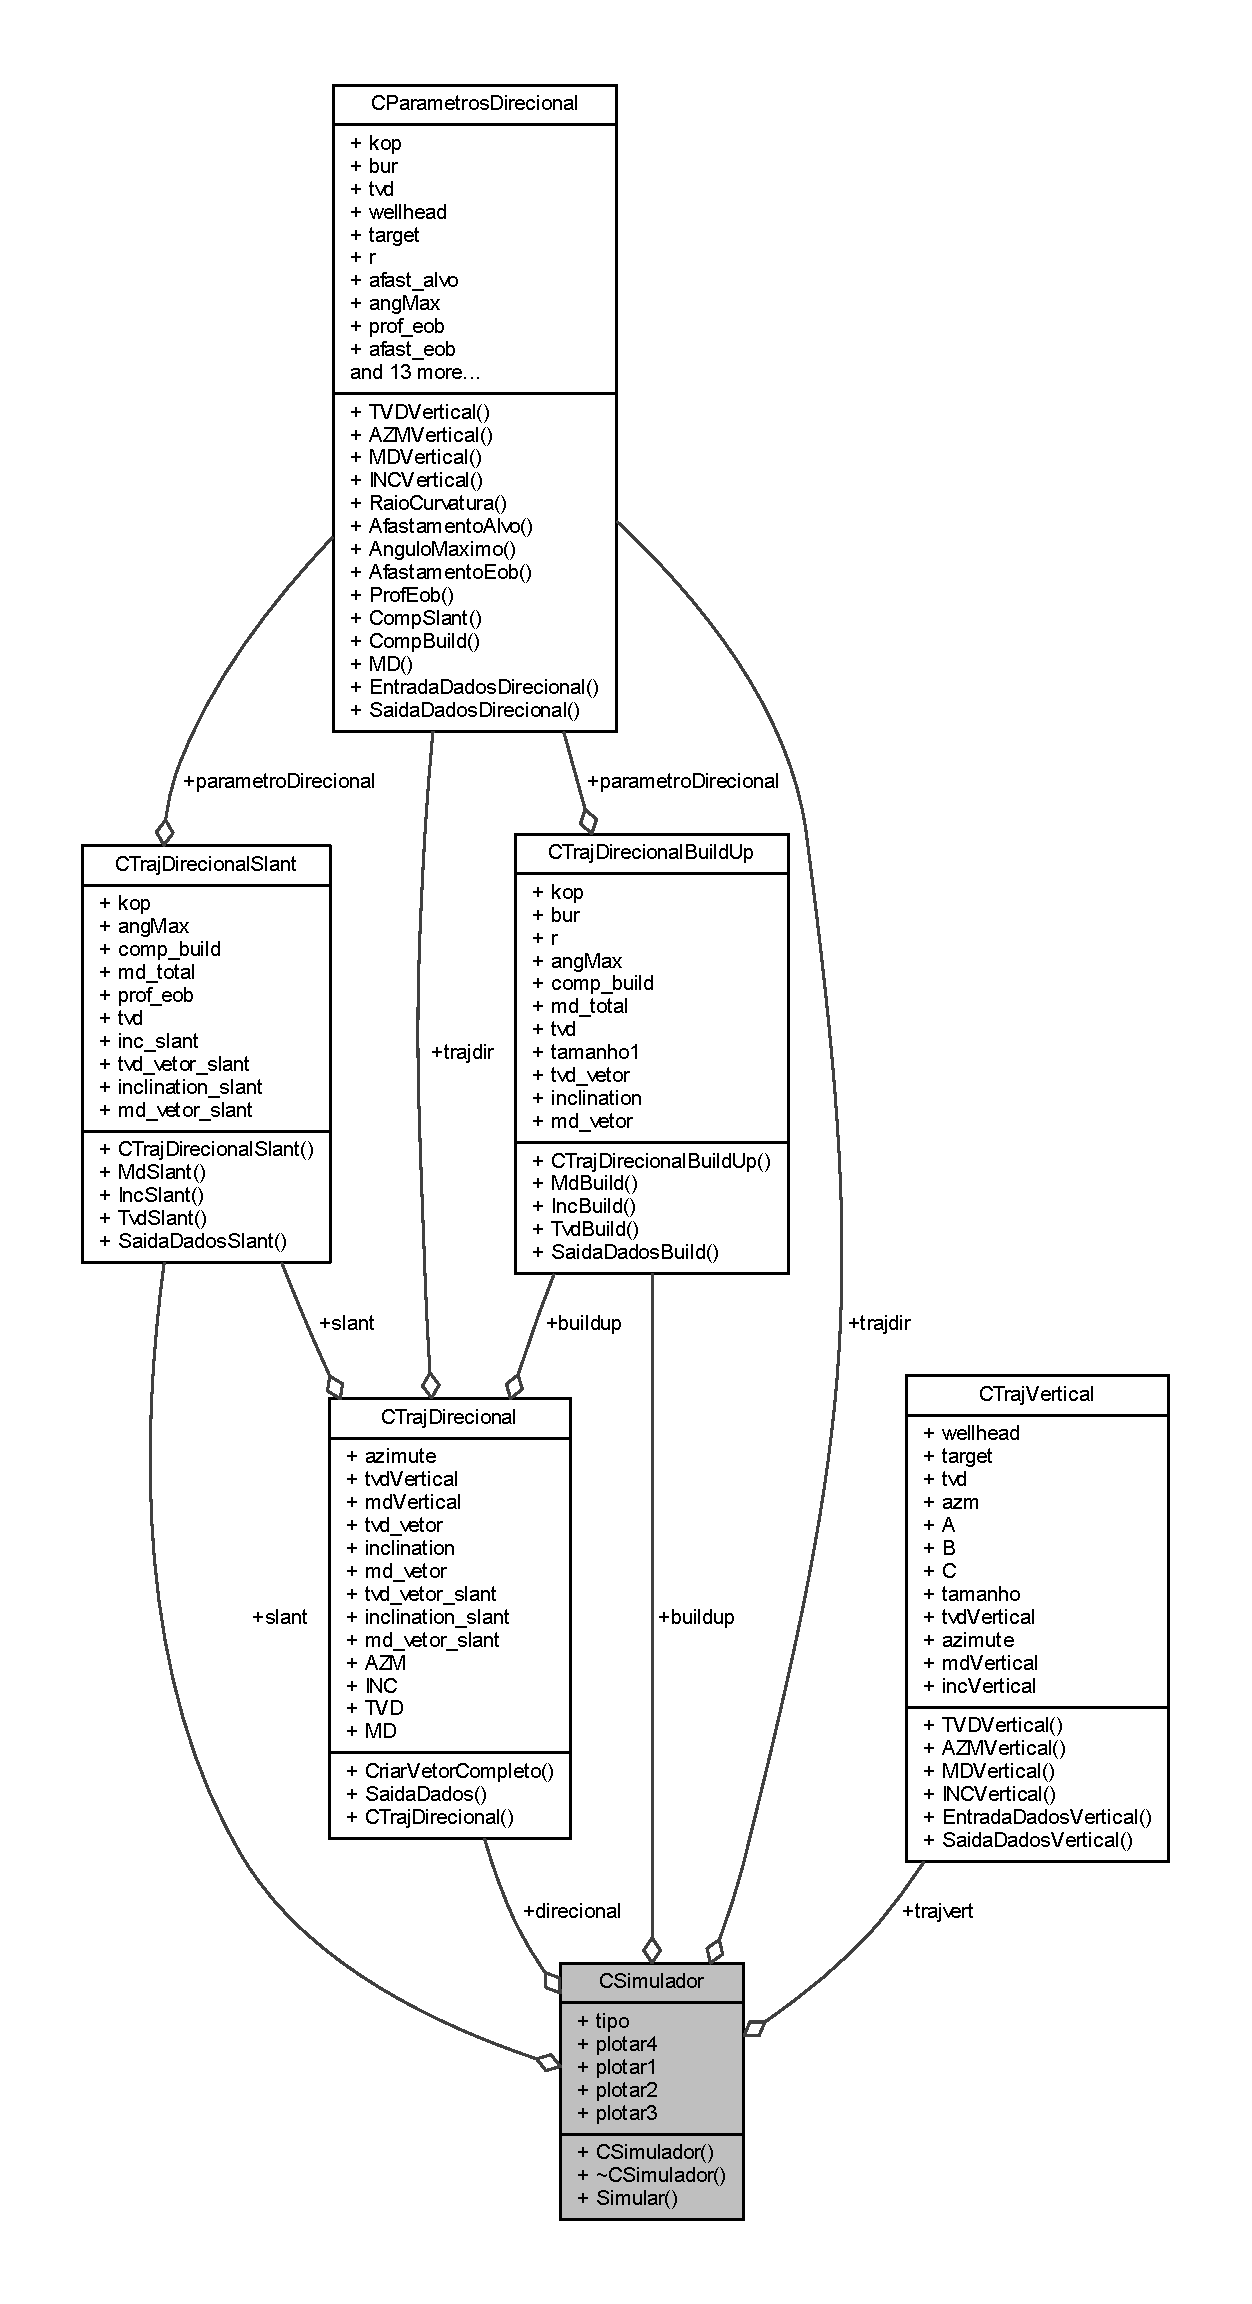
\includegraphics[height=550pt]{class_c_simulador__coll__graph}
\end{center}
\end{figure}
\subsection*{Public Member Functions}
\begin{DoxyCompactItemize}
\item 
\hyperlink{class_c_simulador_aa5abf5e65b423714d5bab7f645d36b77}{C\+Simulador} ()
\item 
virtual \hyperlink{class_c_simulador_ab60fc7dcf2235d3f804a40f1d571a62f}{$\sim$\+C\+Simulador} ()
\item 
void \hyperlink{class_c_simulador_a4f6b4bcb12c412dd65b44c2001c26db8}{Simular} ()
\end{DoxyCompactItemize}
\subsection*{Public Attributes}
\begin{DoxyCompactItemize}
\item 
\mbox{\Hypertarget{class_c_simulador_af07efb956d9bc013d0c6c5f5269fbc50}\label{class_c_simulador_af07efb956d9bc013d0c6c5f5269fbc50}} 
char \hyperlink{class_c_simulador_af07efb956d9bc013d0c6c5f5269fbc50}{tipo}
\begin{DoxyCompactList}\small\item\em M�\+T\+O\+DO DA C\+L\+A\+S\+SE. \end{DoxyCompactList}\item 
\mbox{\Hypertarget{class_c_simulador_a2c330c36780f9df130a61976ad098507}\label{class_c_simulador_a2c330c36780f9df130a61976ad098507}} 
C\+Gnuplot \hyperlink{class_c_simulador_a2c330c36780f9df130a61976ad098507}{plotar4}
\begin{DoxyCompactList}\small\item\em V\+A\+R\+I�\+V\+EL U\+T\+I\+L\+I\+Z\+A\+DA P\+A\+RA D\+E\+T\+E\+R\+M\+I\+N\+AR O T\+I\+PO DO P\+O�O \end{DoxyCompactList}\item 
\mbox{\Hypertarget{class_c_simulador_a3afbc3d56f9648bc10fd0cc1f611385f}\label{class_c_simulador_a3afbc3d56f9648bc10fd0cc1f611385f}} 
C\+Gnuplot \hyperlink{class_c_simulador_a3afbc3d56f9648bc10fd0cc1f611385f}{plotar1}
\begin{DoxyCompactList}\small\item\em O\+B\+J\+E\+T\+OS U\+T\+I\+L\+I\+Z\+A\+D\+OS P\+A\+RA C\+R\+I\+AR OS T\+R�S G\+R�\+F\+I\+C\+OS. \end{DoxyCompactList}\item 
\mbox{\Hypertarget{class_c_simulador_a8a54da0c02bb9500a9a9c529c08c3ca8}\label{class_c_simulador_a8a54da0c02bb9500a9a9c529c08c3ca8}} 
C\+Gnuplot {\bfseries plotar2}
\item 
\mbox{\Hypertarget{class_c_simulador_a2abe37a27c258664ad1f5a87da1643cc}\label{class_c_simulador_a2abe37a27c258664ad1f5a87da1643cc}} 
C\+Gnuplot {\bfseries plotar3}
\item 
\mbox{\Hypertarget{class_c_simulador_aa1a5680c87fbabd02b11718183578e06}\label{class_c_simulador_aa1a5680c87fbabd02b11718183578e06}} 
\hyperlink{class_c_traj_vertical}{C\+Traj\+Vertical} $\ast$ {\bfseries trajvert}
\item 
\mbox{\Hypertarget{class_c_simulador_aa90933bca5f5520dac324744de418e49}\label{class_c_simulador_aa90933bca5f5520dac324744de418e49}} 
\hyperlink{class_c_parametros_direcional}{C\+Parametros\+Direcional} $\ast$ \hyperlink{class_c_simulador_aa90933bca5f5520dac324744de418e49}{trajdir}
\begin{DoxyCompactList}\small\item\em P\+O\+N\+T\+E\+I\+R\+OS C\+R\+I\+A\+D\+OS Q\+UE A\+P\+O\+N\+T\+AM P\+A\+RA OS O\+B\+J\+E\+T\+OS D\+AS C\+L\+A\+S\+S\+ES. \end{DoxyCompactList}\item 
\mbox{\Hypertarget{class_c_simulador_a0a8acab4474cbc3cd31a2bd5877a19a0}\label{class_c_simulador_a0a8acab4474cbc3cd31a2bd5877a19a0}} 
\hyperlink{class_c_traj_direcional_build_up}{C\+Traj\+Direcional\+Build\+Up} $\ast$ {\bfseries buildup}
\item 
\mbox{\Hypertarget{class_c_simulador_abd7c342b877809b52d3499d60fd4ac6f}\label{class_c_simulador_abd7c342b877809b52d3499d60fd4ac6f}} 
\hyperlink{class_c_traj_direcional_slant}{C\+Traj\+Direcional\+Slant} $\ast$ {\bfseries slant}
\item 
\mbox{\Hypertarget{class_c_simulador_a7fd669d5c43b4dfebace5dc9b222e17f}\label{class_c_simulador_a7fd669d5c43b4dfebace5dc9b222e17f}} 
\hyperlink{class_c_traj_direcional}{C\+Traj\+Direcional} $\ast$ {\bfseries direcional}
\end{DoxyCompactItemize}


\subsection{Detailed Description}
O S\+I\+M\+U\+L\+A\+D\+OR R\+E\+U\+N\+IE T\+O\+D\+AS AS C\+L\+A\+S\+S\+ES E A\+C\+E\+S\+SA T\+O\+D\+AS P\+A\+RA C\+H\+A\+M\+AR OS R\+E\+S\+U\+L\+T\+A\+D\+OS. 

\subsection{Constructor \& Destructor Documentation}
\mbox{\Hypertarget{class_c_simulador_aa5abf5e65b423714d5bab7f645d36b77}\label{class_c_simulador_aa5abf5e65b423714d5bab7f645d36b77}} 
\index{C\+Simulador@{C\+Simulador}!C\+Simulador@{C\+Simulador}}
\index{C\+Simulador@{C\+Simulador}!C\+Simulador@{C\+Simulador}}
\subsubsection{\texorpdfstring{C\+Simulador()}{CSimulador()}}
{\footnotesize\ttfamily C\+Simulador\+::\+C\+Simulador (\begin{DoxyParamCaption}{ }\end{DoxyParamCaption})\hspace{0.3cm}{\ttfamily [inline]}}

C\+O\+N\+S\+T\+R\+U\+T\+OR DO S\+I\+M\+U\+L\+A\+D\+OR E D\+OS O\+B\+J\+E\+T\+OS \mbox{\Hypertarget{class_c_simulador_ab60fc7dcf2235d3f804a40f1d571a62f}\label{class_c_simulador_ab60fc7dcf2235d3f804a40f1d571a62f}} 
\index{C\+Simulador@{C\+Simulador}!````~C\+Simulador@{$\sim$\+C\+Simulador}}
\index{````~C\+Simulador@{$\sim$\+C\+Simulador}!C\+Simulador@{C\+Simulador}}
\subsubsection{\texorpdfstring{$\sim$\+C\+Simulador()}{~CSimulador()}}
{\footnotesize\ttfamily virtual C\+Simulador\+::$\sim$\+C\+Simulador (\begin{DoxyParamCaption}{ }\end{DoxyParamCaption})\hspace{0.3cm}{\ttfamily [inline]}, {\ttfamily [virtual]}}

D\+E\+S\+T\+R\+U\+T\+OR DE T\+O\+D\+OS OS O\+B\+J\+E\+T\+OS J\+U\+N\+TO C\+OM A C\+L\+A\+S\+SE Here is the call graph for this function\+:
\nopagebreak
\begin{figure}[H]
\begin{center}
\leavevmode
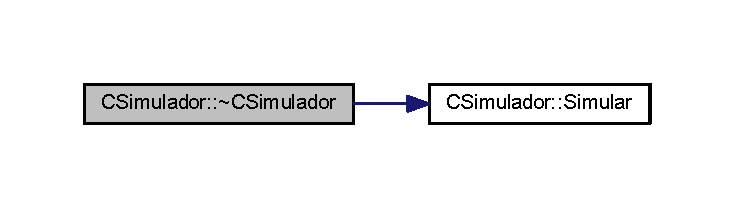
\includegraphics[width=350pt]{class_c_simulador_ab60fc7dcf2235d3f804a40f1d571a62f_cgraph}
\end{center}
\end{figure}


\subsection{Member Function Documentation}
\mbox{\Hypertarget{class_c_simulador_a4f6b4bcb12c412dd65b44c2001c26db8}\label{class_c_simulador_a4f6b4bcb12c412dd65b44c2001c26db8}} 
\index{C\+Simulador@{C\+Simulador}!Simular@{Simular}}
\index{Simular@{Simular}!C\+Simulador@{C\+Simulador}}
\subsubsection{\texorpdfstring{Simular()}{Simular()}}
{\footnotesize\ttfamily void C\+Simulador\+::\+Simular (\begin{DoxyParamCaption}{ }\end{DoxyParamCaption})}

C\+A\+B\+E�\+A\+L\+HO DO N\+O\+S\+SO P\+R\+O\+G\+R\+A\+MA

A\+Q\+UI O U\+S\+U�\+R\+IO E\+S\+C\+O\+L\+HE O T\+I\+PO DO P\+O�O

M\+E\+N\+S\+A\+G\+EM DE E\+R\+RO C\+A\+SO O U\+S\+U�\+R\+IO D\+I\+G\+I\+T\+AR A\+L\+GO N�O

E\+S\+P\+E\+R\+A\+DO

C\+A\+SO O U\+S\+U�\+R\+IO E\+S\+C\+O\+L\+HA V P\+A\+RA P\+O�O V\+E\+R\+T\+I\+C\+AL, E\+N\+T\+R\+A\+M\+OS N\+E\+S\+SA R\+O\+T\+I\+NA

entra atributos independentes e calcula atributos dependentes

N\+E\+S\+TA P\+A\+R\+TE DO N\+O\+S\+SO C�\+D\+I\+GO G\+E\+R\+A\+M\+OS OS G\+R�\+F\+I\+C\+OS N\+E\+C\+E\+S\+S�\+R\+I\+OS P\+A\+RA A\+N�\+L\+I\+SE D\+OS R\+E\+S\+U\+L\+T\+A\+D\+OS

SE E\+S\+C\+O\+L\+H\+ER UM P\+O�O D\+I\+R\+E\+C\+I\+O\+N\+AL, E\+N\+T\+R\+A\+M\+OS N\+E\+S\+SA R\+O\+T\+I\+NA

entra atributos independentes e calcula atributos dependentes

N\+E\+S\+TA P\+A\+R\+TE DO N\+O\+S\+SO C�\+D\+I\+GO G\+E\+R\+A\+M\+OS OS G\+R�\+F\+I\+C\+OS N\+E\+C\+E\+S\+S�\+R\+I\+OS P\+A\+RA A\+N�\+L\+I\+SE D\+OS R\+E\+S\+U\+L\+T\+A\+D\+OS Here is the caller graph for this function\+:
\nopagebreak
\begin{figure}[H]
\begin{center}
\leavevmode
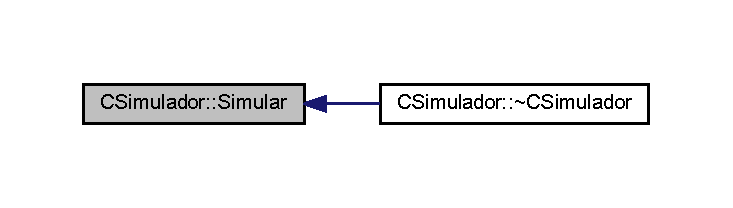
\includegraphics[width=350pt]{class_c_simulador_a4f6b4bcb12c412dd65b44c2001c26db8_icgraph}
\end{center}
\end{figure}


The documentation for this class was generated from the following files\+:\begin{DoxyCompactItemize}
\item 
C\+Simulador.\+h\item 
C\+Simulador.\+cpp\end{DoxyCompactItemize}

\hypertarget{class_c_traj_direcional}{}\section{C\+Traj\+Direcional Class Reference}
\label{class_c_traj_direcional}\index{C\+Traj\+Direcional@{C\+Traj\+Direcional}}


P\+A\+RA I\+S\+SO P\+R\+E\+C\+I\+S\+A\+M\+OS I\+N\+C\+L\+U\+IR T\+O\+D\+AS AS C\+L\+A\+S\+S\+ES.  




{\ttfamily \#include $<$C\+Traj\+Direcional.\+h$>$}



Collaboration diagram for C\+Traj\+Direcional\+:
\nopagebreak
\begin{figure}[H]
\begin{center}
\leavevmode
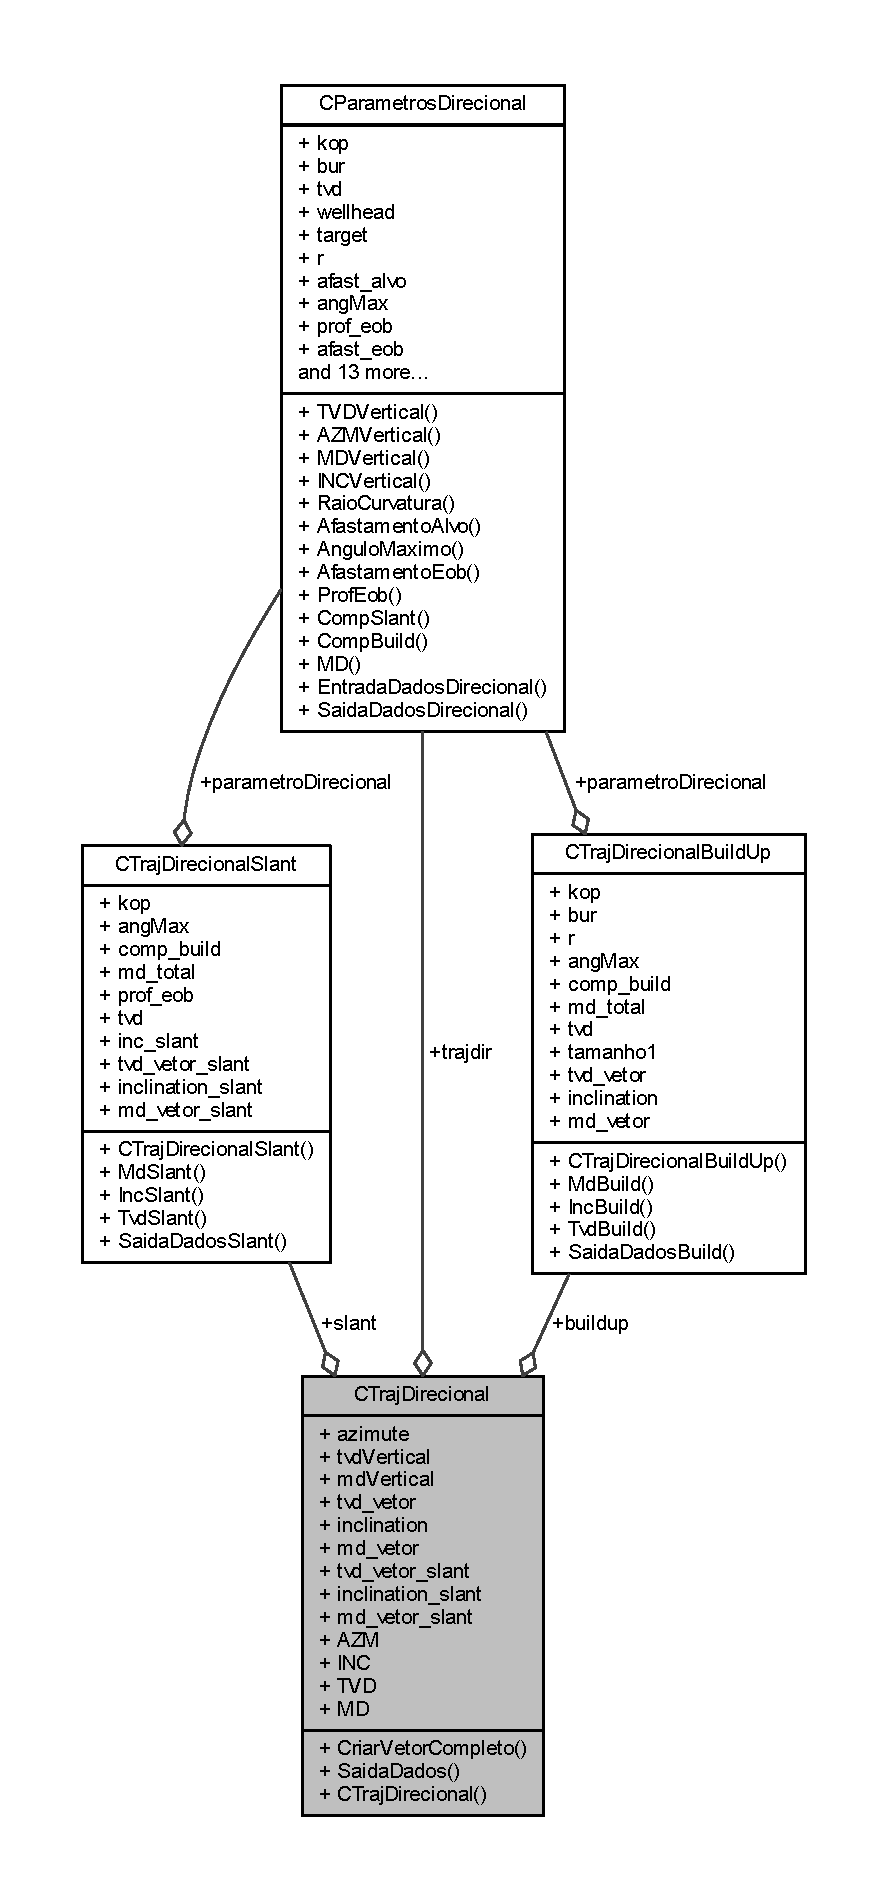
\includegraphics[height=550pt]{class_c_traj_direcional__coll__graph}
\end{center}
\end{figure}
\subsection*{Public Member Functions}
\begin{DoxyCompactItemize}
\item 
void \hyperlink{class_c_traj_direcional_a2b3f2474dccef5849eb09daeab244120}{Criar\+Vetor\+Completo} ()
\item 
void \hyperlink{class_c_traj_direcional_a8aa0c970230082cc529c5925281079dd}{Saida\+Dados} ()
\begin{DoxyCompactList}\small\item\em M�\+T\+O\+D\+OS DA C\+L\+A\+S\+SE. \end{DoxyCompactList}\item 
\mbox{\Hypertarget{class_c_traj_direcional_a5c79f98c1ea23a19d37d4f243f34e139}\label{class_c_traj_direcional_a5c79f98c1ea23a19d37d4f243f34e139}} 
{\bfseries C\+Traj\+Direcional} (\hyperlink{class_c_parametros_direcional}{C\+Parametros\+Direcional} $\ast$\+\_\+trajdir, \hyperlink{class_c_traj_direcional_build_up}{C\+Traj\+Direcional\+Build\+Up} $\ast$\+\_\+buildup, \hyperlink{class_c_traj_direcional_slant}{C\+Traj\+Direcional\+Slant} $\ast$\+\_\+slant)
\end{DoxyCompactItemize}
\subsection*{Public Attributes}
\begin{DoxyCompactItemize}
\item 
\mbox{\Hypertarget{class_c_traj_direcional_adc483b95622385fc046dc7828644f08b}\label{class_c_traj_direcional_adc483b95622385fc046dc7828644f08b}} 
std\+::vector$<$ double $>$ {\bfseries azimute}
\item 
\mbox{\Hypertarget{class_c_traj_direcional_aac58891fa3b5478abf4ca414c11fb7a0}\label{class_c_traj_direcional_aac58891fa3b5478abf4ca414c11fb7a0}} 
std\+::vector$<$ double $>$ \hyperlink{class_c_traj_direcional_aac58891fa3b5478abf4ca414c11fb7a0}{tvd\+Vertical}
\begin{DoxyCompactList}\small\item\em V\+E\+T\+O\+R\+ES DA S\+E��O V\+E\+R\+T\+I\+C\+AL. \end{DoxyCompactList}\item 
\mbox{\Hypertarget{class_c_traj_direcional_a9196e75d71015e08d95236e69bad2493}\label{class_c_traj_direcional_a9196e75d71015e08d95236e69bad2493}} 
std\+::vector$<$ double $>$ {\bfseries md\+Vertical}
\item 
\mbox{\Hypertarget{class_c_traj_direcional_a300f2e02b3c9c8a8cc5faa4216c1d9e5}\label{class_c_traj_direcional_a300f2e02b3c9c8a8cc5faa4216c1d9e5}} 
std\+::vector$<$ double $>$ {\bfseries tvd\+\_\+vetor}
\item 
\mbox{\Hypertarget{class_c_traj_direcional_abd5ad465041db23080667e9545351d8a}\label{class_c_traj_direcional_abd5ad465041db23080667e9545351d8a}} 
std\+::vector$<$ double $>$ \hyperlink{class_c_traj_direcional_abd5ad465041db23080667e9545351d8a}{inclination}
\begin{DoxyCompactList}\small\item\em V\+E\+T\+O\+R\+ES DA S\+E��O B\+U\+I\+LD (G\+A\+N\+HO DE �\+N\+G\+U\+LO) \end{DoxyCompactList}\item 
\mbox{\Hypertarget{class_c_traj_direcional_ae3363071d6bae02046db05ea9664ee22}\label{class_c_traj_direcional_ae3363071d6bae02046db05ea9664ee22}} 
std\+::vector$<$ double $>$ {\bfseries md\+\_\+vetor}
\item 
\mbox{\Hypertarget{class_c_traj_direcional_a8050dde8e3ff80f1cfbe549f4a70d457}\label{class_c_traj_direcional_a8050dde8e3ff80f1cfbe549f4a70d457}} 
std\+::vector$<$ double $>$ {\bfseries tvd\+\_\+vetor\+\_\+slant}
\item 
\mbox{\Hypertarget{class_c_traj_direcional_a61b65bb1fdb90cd31aca81a03ac5c71c}\label{class_c_traj_direcional_a61b65bb1fdb90cd31aca81a03ac5c71c}} 
std\+::vector$<$ double $>$ \hyperlink{class_c_traj_direcional_a61b65bb1fdb90cd31aca81a03ac5c71c}{inclination\+\_\+slant}
\begin{DoxyCompactList}\small\item\em V\+E\+T\+O\+R\+ES DA S\+E��O S\+L\+A\+NT (T\+A\+N\+G\+E\+N\+TE) \end{DoxyCompactList}\item 
\mbox{\Hypertarget{class_c_traj_direcional_a8c1123d97383584608ab49e11859a57e}\label{class_c_traj_direcional_a8c1123d97383584608ab49e11859a57e}} 
std\+::vector$<$ double $>$ {\bfseries md\+\_\+vetor\+\_\+slant}
\item 
\mbox{\Hypertarget{class_c_traj_direcional_a78ccc521be60bbf56080c771d1244538}\label{class_c_traj_direcional_a78ccc521be60bbf56080c771d1244538}} 
std\+::vector$<$ double $>$ {\bfseries A\+ZM}
\item 
\mbox{\Hypertarget{class_c_traj_direcional_a67a2f3b888e74cc1b8560965d046593d}\label{class_c_traj_direcional_a67a2f3b888e74cc1b8560965d046593d}} 
std\+::vector$<$ double $>$ \hyperlink{class_c_traj_direcional_a67a2f3b888e74cc1b8560965d046593d}{I\+NC}
\begin{DoxyCompactList}\small\item\em V\+E\+T\+O\+R\+ES C\+O\+N\+C\+A\+T\+E\+N\+A\+D\+OS, E\+X\+I\+B\+I\+N\+DO OS R\+E\+S\+U\+L\+T\+A\+D\+OS DA T\+R\+A\+J\+E\+T�\+R\+IA C\+O\+M\+P\+L\+E\+TA DO P\+O�O \end{DoxyCompactList}\item 
\mbox{\Hypertarget{class_c_traj_direcional_aba4fe1548eceb19ae7b41d574ee5d9c7}\label{class_c_traj_direcional_aba4fe1548eceb19ae7b41d574ee5d9c7}} 
std\+::vector$<$ double $>$ {\bfseries T\+VD}
\item 
\mbox{\Hypertarget{class_c_traj_direcional_a9d5750df1c50d012cc96c8b5aef5cb3f}\label{class_c_traj_direcional_a9d5750df1c50d012cc96c8b5aef5cb3f}} 
std\+::vector$<$ double $>$ {\bfseries MD}
\item 
\mbox{\Hypertarget{class_c_traj_direcional_a1f81697b9f52cde4e30950119e77ebbf}\label{class_c_traj_direcional_a1f81697b9f52cde4e30950119e77ebbf}} 
\hyperlink{class_c_parametros_direcional}{C\+Parametros\+Direcional} $\ast$ {\bfseries trajdir}
\item 
\mbox{\Hypertarget{class_c_traj_direcional_a12416e268010c748e1987b157758444f}\label{class_c_traj_direcional_a12416e268010c748e1987b157758444f}} 
\hyperlink{class_c_traj_direcional_build_up}{C\+Traj\+Direcional\+Build\+Up} $\ast$ \hyperlink{class_c_traj_direcional_a12416e268010c748e1987b157758444f}{buildup}
\begin{DoxyCompactList}\small\item\em O\+B\+J\+E\+T\+OS C\+R\+I\+A\+D\+OS P\+A\+RA U\+T\+I\+L\+I\+Z\+AR OS V\+E\+T\+O\+R\+ES D\+AS O\+U\+T\+R\+AS C\+L\+A\+S\+S\+ES. \end{DoxyCompactList}\item 
\mbox{\Hypertarget{class_c_traj_direcional_a495cd405e0aba144f3d3241865645dda}\label{class_c_traj_direcional_a495cd405e0aba144f3d3241865645dda}} 
\hyperlink{class_c_traj_direcional_slant}{C\+Traj\+Direcional\+Slant} $\ast$ {\bfseries slant}
\end{DoxyCompactItemize}


\subsection{Detailed Description}
P\+A\+RA I\+S\+SO P\+R\+E\+C\+I\+S\+A\+M\+OS I\+N\+C\+L\+U\+IR T\+O\+D\+AS AS C\+L\+A\+S\+S\+ES. 

C\+L\+A\+S\+SE C\+R\+I\+A\+DA P\+A\+RA C\+O\+N\+C\+A\+T\+E\+N\+AR T\+O\+D\+OS OS V\+E\+T\+O\+R\+ES C\+R\+I\+A\+D\+OS E M\+O\+S\+T\+R\+AR O R\+E\+S\+U\+L\+T\+A\+DO DE T\+O\+DA A T\+R\+A\+J\+E\+T�\+R\+IA DO P\+O�O 

\subsection{Member Function Documentation}
\mbox{\Hypertarget{class_c_traj_direcional_a2b3f2474dccef5849eb09daeab244120}\label{class_c_traj_direcional_a2b3f2474dccef5849eb09daeab244120}} 
\index{C\+Traj\+Direcional@{C\+Traj\+Direcional}!Criar\+Vetor\+Completo@{Criar\+Vetor\+Completo}}
\index{Criar\+Vetor\+Completo@{Criar\+Vetor\+Completo}!C\+Traj\+Direcional@{C\+Traj\+Direcional}}
\subsubsection{\texorpdfstring{Criar\+Vetor\+Completo()}{CriarVetorCompleto()}}
{\footnotesize\ttfamily void C\+Traj\+Direcional\+::\+Criar\+Vetor\+Completo (\begin{DoxyParamCaption}{ }\end{DoxyParamCaption})}

V\+E\+T\+OR T\+VD

V\+E\+T\+OR MD

V\+E\+T\+OR I\+NC

V\+E\+T\+OR A\+ZM

A\+Q\+UI J\+O\+G\+A\+M\+OS O R\+E\+S\+U\+L\+T\+A\+DO NA T\+E\+LA EM C\+O\+L\+U\+N\+AS \mbox{\Hypertarget{class_c_traj_direcional_a8aa0c970230082cc529c5925281079dd}\label{class_c_traj_direcional_a8aa0c970230082cc529c5925281079dd}} 
\index{C\+Traj\+Direcional@{C\+Traj\+Direcional}!Saida\+Dados@{Saida\+Dados}}
\index{Saida\+Dados@{Saida\+Dados}!C\+Traj\+Direcional@{C\+Traj\+Direcional}}
\subsubsection{\texorpdfstring{Saida\+Dados()}{SaidaDados()}}
{\footnotesize\ttfamily void C\+Traj\+Direcional\+::\+Saida\+Dados (\begin{DoxyParamCaption}{ }\end{DoxyParamCaption})}



M�\+T\+O\+D\+OS DA C\+L\+A\+S\+SE. 

A\+R\+Q\+U\+I\+VO C\+OM A T\+A\+B\+E\+LA D\+OS R\+E\+S\+U\+L\+T\+A\+D\+OS F\+I\+N\+A\+IS DO P\+R\+O\+G\+R\+A\+MA 

The documentation for this class was generated from the following files\+:\begin{DoxyCompactItemize}
\item 
C\+Traj\+Direcional.\+h\item 
C\+Traj\+Direcional.\+cpp\end{DoxyCompactItemize}

\hypertarget{class_c_traj_direcional_build_up}{}\section{C\+Traj\+Direcional\+Build\+Up Class Reference}
\label{class_c_traj_direcional_build_up}\index{C\+Traj\+Direcional\+Build\+Up@{C\+Traj\+Direcional\+Build\+Up}}


U\+T\+I\+L\+I\+Z\+AR OS P\+A\+RÂ\+M\+E\+T\+R\+OS D\+I\+R\+E\+C\+I\+O\+N\+A\+IS C\+A\+L\+C\+U\+L\+A\+D\+OS NA C\+L\+A\+S\+SE \char`\"{}\+C\+P\+A\+R\+A\+M\+E\+T\+R\+O\+S\+D\+I\+R\+E\+C\+I\+O\+N\+A\+L\char`\"{}.  




{\ttfamily \#include $<$C\+Traj\+Direcional\+Build\+Up.\+h$>$}



Collaboration diagram for C\+Traj\+Direcional\+Build\+Up\+:
\nopagebreak
\begin{figure}[H]
\begin{center}
\leavevmode
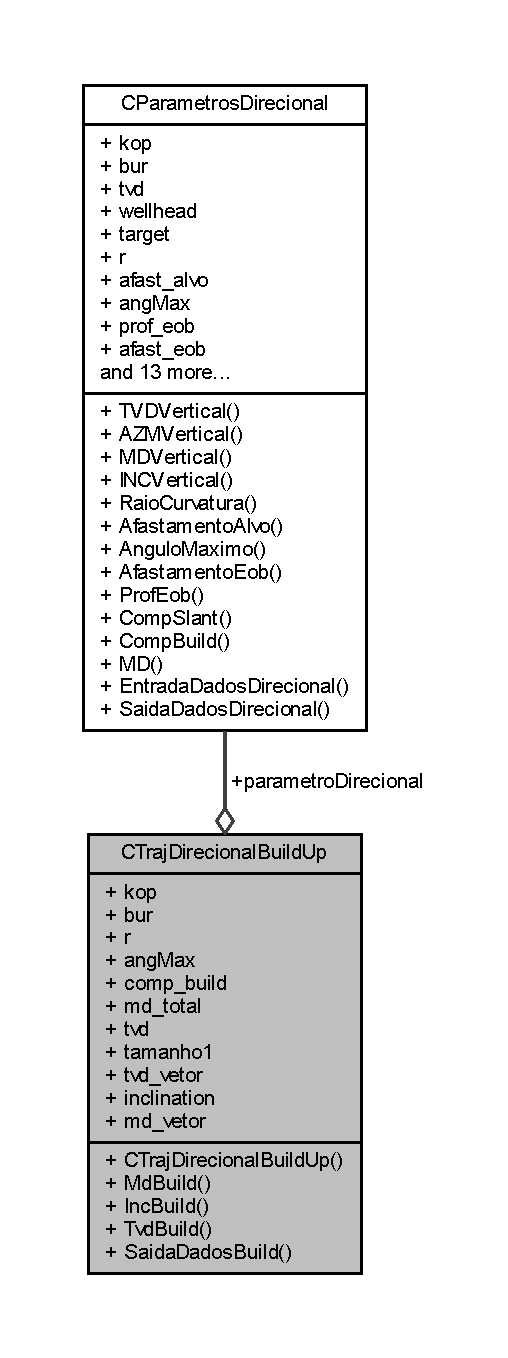
\includegraphics[height=550pt]{class_c_traj_direcional_build_up__coll__graph}
\end{center}
\end{figure}
\subsection*{Public Member Functions}
\begin{DoxyCompactItemize}
\item 
\mbox{\Hypertarget{class_c_traj_direcional_build_up_aa902c99af4da0ff0f4ec1a64aeb32692}\label{class_c_traj_direcional_build_up_aa902c99af4da0ff0f4ec1a64aeb32692}} 
\hyperlink{class_c_traj_direcional_build_up_aa902c99af4da0ff0f4ec1a64aeb32692}{C\+Traj\+Direcional\+Build\+Up} (\hyperlink{class_c_parametros_direcional}{C\+Parametros\+Direcional} $\ast$\+\_\+parametro\+Direcional)
\begin{DoxyCompactList}\small\item\em C\+O\+N\+S\+T\+R\+U\+T\+OR C\+H\+A\+M\+A\+N\+DO P\+OR P\+O\+N\+T\+E\+I\+RO OS O\+B\+J\+E\+T\+OS C\+R\+I\+A\+D\+OS. \end{DoxyCompactList}\item 
void \hyperlink{class_c_traj_direcional_build_up_a386a6f7a05072e1ed6e8edc310e77a90}{Md\+Build} ()
\item 
void \hyperlink{class_c_traj_direcional_build_up_a4e7b281295b9d336e677992a7c0b2bd9}{Inc\+Build} ()
\begin{DoxyCompactList}\small\item\em MÉ\+T\+O\+D\+OS DA C\+L\+A\+S\+SE. \end{DoxyCompactList}\item 
void \hyperlink{class_c_traj_direcional_build_up_a45fb72046a3a4ee60d9ff902a63c866c}{Tvd\+Build} ()
\item 
void \hyperlink{class_c_traj_direcional_build_up_a8f6f8b3419d26a90601ec7b74c7b137a}{Saida\+Dados\+Build} ()
\end{DoxyCompactItemize}
\subsection*{Public Attributes}
\begin{DoxyCompactItemize}
\item 
\mbox{\Hypertarget{class_c_traj_direcional_build_up_ae05e10eed4ea237cdc905737f07097df}\label{class_c_traj_direcional_build_up_ae05e10eed4ea237cdc905737f07097df}} 
double {\bfseries kop}
\item 
\mbox{\Hypertarget{class_c_traj_direcional_build_up_ab16523998221ca38f06b9c1fb5f4a242}\label{class_c_traj_direcional_build_up_ab16523998221ca38f06b9c1fb5f4a242}} 
double \hyperlink{class_c_traj_direcional_build_up_ab16523998221ca38f06b9c1fb5f4a242}{bur}
\begin{DoxyCompactList}\small\item\em A\+Q\+UI C\+H\+A\+M\+A\+M\+OS OS P\+A\+RÂ\+M\+E\+T\+R\+OS C\+A\+L\+C\+U\+L\+A\+D\+OS NA O\+U\+T\+RA C\+L\+A\+S\+SE Q\+UE S\+E\+RÃO U\+T\+I\+L\+I\+Z\+A\+D\+OS NO CÁ\+L\+C\+U\+LO D\+OS V\+E\+T\+O\+R\+ES. \end{DoxyCompactList}\item 
\mbox{\Hypertarget{class_c_traj_direcional_build_up_a008d5f2cb5a1b8c0ff20dafd6e1d2a75}\label{class_c_traj_direcional_build_up_a008d5f2cb5a1b8c0ff20dafd6e1d2a75}} 
double {\bfseries r}
\item 
\mbox{\Hypertarget{class_c_traj_direcional_build_up_acbdd303c696ea797b09bc7e7a8c51742}\label{class_c_traj_direcional_build_up_acbdd303c696ea797b09bc7e7a8c51742}} 
double {\bfseries ang\+Max}
\item 
\mbox{\Hypertarget{class_c_traj_direcional_build_up_a6b9d69817429df71cd601f564583b85f}\label{class_c_traj_direcional_build_up_a6b9d69817429df71cd601f564583b85f}} 
double {\bfseries comp\+\_\+build}
\item 
\mbox{\Hypertarget{class_c_traj_direcional_build_up_a5c6a71222a0414a25d65c4816a02107f}\label{class_c_traj_direcional_build_up_a5c6a71222a0414a25d65c4816a02107f}} 
double {\bfseries md\+\_\+total}
\item 
\mbox{\Hypertarget{class_c_traj_direcional_build_up_a9c5deba522ae74a9de89026c48cf1cd6}\label{class_c_traj_direcional_build_up_a9c5deba522ae74a9de89026c48cf1cd6}} 
double {\bfseries tvd}
\item 
\mbox{\Hypertarget{class_c_traj_direcional_build_up_a47ca0fccc68cf311001ff440b2312721}\label{class_c_traj_direcional_build_up_a47ca0fccc68cf311001ff440b2312721}} 
int {\bfseries tamanho1}
\item 
\mbox{\Hypertarget{class_c_traj_direcional_build_up_a23dda15b44241c9bdb8c80fcba322f23}\label{class_c_traj_direcional_build_up_a23dda15b44241c9bdb8c80fcba322f23}} 
std\+::vector$<$ double $>$ {\bfseries tvd\+\_\+vetor}
\item 
\mbox{\Hypertarget{class_c_traj_direcional_build_up_af0717036156f18b45fcbf078c3b91a01}\label{class_c_traj_direcional_build_up_af0717036156f18b45fcbf078c3b91a01}} 
std\+::vector$<$ double $>$ \hyperlink{class_c_traj_direcional_build_up_af0717036156f18b45fcbf078c3b91a01}{inclination}
\begin{DoxyCompactList}\small\item\em V\+E\+T\+O\+R\+ES Q\+UE S\+E\+RÃO C\+R\+I\+A\+D\+OS N\+E\+S\+SA C\+L\+A\+S\+SE P\+A\+RA R\+E\+P\+R\+E\+S\+E\+N\+T\+AR A T\+R\+A\+J\+E\+TÓ\+R\+IA DE G\+A\+N\+HO DE Â\+N\+G\+U\+LO. \end{DoxyCompactList}\item 
\mbox{\Hypertarget{class_c_traj_direcional_build_up_a105cdccf6ea75d61b7a10669fdb7381b}\label{class_c_traj_direcional_build_up_a105cdccf6ea75d61b7a10669fdb7381b}} 
std\+::vector$<$ double $>$ {\bfseries md\+\_\+vetor}
\item 
\mbox{\Hypertarget{class_c_traj_direcional_build_up_a254e85f61f26a325a44d90265852fc88}\label{class_c_traj_direcional_build_up_a254e85f61f26a325a44d90265852fc88}} 
\hyperlink{class_c_parametros_direcional}{C\+Parametros\+Direcional} $\ast$ {\bfseries parametro\+Direcional}
\end{DoxyCompactItemize}


\subsection{Detailed Description}
U\+T\+I\+L\+I\+Z\+AR OS P\+A\+RÂ\+M\+E\+T\+R\+OS D\+I\+R\+E\+C\+I\+O\+N\+A\+IS C\+A\+L\+C\+U\+L\+A\+D\+OS NA C\+L\+A\+S\+SE \char`\"{}\+C\+P\+A\+R\+A\+M\+E\+T\+R\+O\+S\+D\+I\+R\+E\+C\+I\+O\+N\+A\+L\char`\"{}. 

E\+S\+SA C\+L\+A\+S\+SE C\+R\+IA A T\+R\+A\+J\+E\+TÓ\+R\+IA DA S\+EÇÃO DE G\+A\+N\+HO DE Â\+N\+G\+U\+LO, P\+A\+RA I\+S\+SO P\+R\+E\+C\+I\+S\+A\+M\+OS 

\subsection{Member Function Documentation}
\mbox{\Hypertarget{class_c_traj_direcional_build_up_a4e7b281295b9d336e677992a7c0b2bd9}\label{class_c_traj_direcional_build_up_a4e7b281295b9d336e677992a7c0b2bd9}} 
\index{C\+Traj\+Direcional\+Build\+Up@{C\+Traj\+Direcional\+Build\+Up}!Inc\+Build@{Inc\+Build}}
\index{Inc\+Build@{Inc\+Build}!C\+Traj\+Direcional\+Build\+Up@{C\+Traj\+Direcional\+Build\+Up}}
\subsubsection{\texorpdfstring{Inc\+Build()}{IncBuild()}}
{\footnotesize\ttfamily void C\+Traj\+Direcional\+Build\+Up\+::\+Inc\+Build (\begin{DoxyParamCaption}{ }\end{DoxyParamCaption})}



MÉ\+T\+O\+D\+OS DA C\+L\+A\+S\+SE. 

C\+R\+I\+A��O DO M�\+T\+O\+DO Q\+UE C\+A\+L\+C\+U\+LA O V\+E\+T\+OR DE I\+N\+C\+L\+I\+N\+A��\+ES

P\+R\+I\+M\+E\+I\+RO V\+A\+L\+OR DO V\+E\+T\+OR � 0, P\+O\+R\+Q\+UE � I\+N\+C\+L\+I\+N\+A��O I\+G\+U\+AL A 0

C\+R\+I\+A\+M\+OS UM C\+O\+N\+T\+A\+T\+OR E I\+N\+I\+C\+I\+A\+M\+OS E\+LE C\+OM O V\+A\+L\+OR 0

L�\+G\+I\+CA DA C\+R\+I\+A��O D\+E\+S\+TE V\+E\+T\+OR

A C\+A\+DA P\+A\+S\+SO DO C\+O\+N\+T\+A\+D\+OR A I\+N\+C\+L\+I\+N\+A��O

M\+U\+DA C\+OM B\+UR, A\+T� O A\+N\+G\+U\+LO M\+A\+X\+I\+MO

�\+L\+T\+I\+MO V\+A\+L\+OR DO N\+O\+S\+SO V\+E\+T\+OR T\+EM Q\+UE S\+ER O A\+N\+G\+U\+LO M�\+X\+I\+MO Here is the caller graph for this function\+:
\nopagebreak
\begin{figure}[H]
\begin{center}
\leavevmode
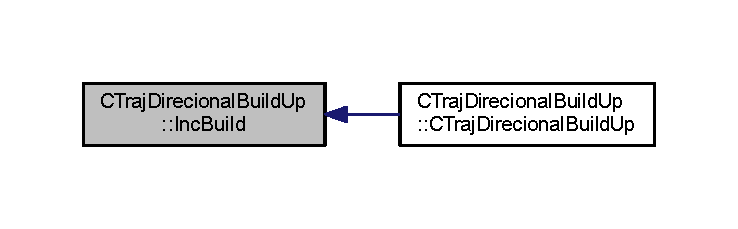
\includegraphics[width=350pt]{class_c_traj_direcional_build_up_a4e7b281295b9d336e677992a7c0b2bd9_icgraph}
\end{center}
\end{figure}
\mbox{\Hypertarget{class_c_traj_direcional_build_up_a386a6f7a05072e1ed6e8edc310e77a90}\label{class_c_traj_direcional_build_up_a386a6f7a05072e1ed6e8edc310e77a90}} 
\index{C\+Traj\+Direcional\+Build\+Up@{C\+Traj\+Direcional\+Build\+Up}!Md\+Build@{Md\+Build}}
\index{Md\+Build@{Md\+Build}!C\+Traj\+Direcional\+Build\+Up@{C\+Traj\+Direcional\+Build\+Up}}
\subsubsection{\texorpdfstring{Md\+Build()}{MdBuild()}}
{\footnotesize\ttfamily void C\+Traj\+Direcional\+Build\+Up\+::\+Md\+Build (\begin{DoxyParamCaption}{ }\end{DoxyParamCaption})}

C\+O\+MO NA S\+E��O DE G\+A\+N\+HO DE �\+N\+G\+U\+LO O N\+O\+S\+SO P\+O�O S\+AI DA V\+E\+R\+T\+I\+C\+AL, P\+R\+E\+C\+I\+S\+A\+M\+OS C\+A\+L\+C\+U\+L\+AR A P\+R\+O\+F\+U\+N\+D\+I\+D\+A\+DE M\+E\+D\+I\+DA D\+E\+LE, P\+A\+RA S\+A\+B\+ER E\+X\+A\+T\+A\+M\+E\+N\+TE A P\+R\+O\+F\+U\+N\+D\+I\+D\+A\+DE P\+E\+R\+C\+O\+R\+R\+I\+DA P\+E\+LO P\+O�O

S\+O\+M\+A\+N\+DO A P\+R\+OF. DE K\+OP C\+OM O C\+O\+M\+P\+R\+I\+M\+E\+N\+TO

DA S\+E��O DE G\+A\+N\+HO, O\+B\+T\+E\+M\+OS O MD A\+T� O F\+I\+N\+AL DA F\+A\+SE

P\+A\+RA N�O S\+O\+B\+R\+E\+P\+OR, A\+U\+M\+E\+N\+T\+A\+M\+OS 10m, P\+O\+R�M C\+O\+MO � I\+N\+C\+L\+I\+N\+A\+DO, U\+T\+I\+L\+I\+Z\+A\+M\+OS O C\+O\+S\+E\+NO P\+A\+RA A\+U\+M\+E\+N\+T\+AR E\+S\+TE P\+A\+S\+SO DE P\+R\+OF.

A\+Q\+UI U\+T\+I\+L\+I\+Z\+A\+M\+OS O N�\+M\+E\+RO DE C\+A\+S\+AS DO V\+E\+T\+OR I\+N\+C\+L\+I\+N\+A��O P\+A\+RA L\+I\+M\+I\+T\+AR E\+S\+SE V\+E\+T\+OR, P\+O\+IS T\+O\+D\+OS V\+E\+T\+O\+R\+ES P\+R\+E\+C\+I\+S\+AM E\+S\+T\+AR NA M\+E\+S\+MA P\+R\+O\+F\+U\+N\+D\+I\+D\+A\+DE E T\+ER O V\+E\+T\+OR DO M\+E\+S\+MO T\+A\+M\+A\+N\+HO

G\+A\+R\+A\+N\+T\+IA Q\+UE O �\+L\+T\+I\+MO V\+A\+L\+OR DO V\+E\+T\+OR � O MD F\+I\+N\+AL D\+E\+S\+TA F\+A\+SE Here is the caller graph for this function\+:
\nopagebreak
\begin{figure}[H]
\begin{center}
\leavevmode
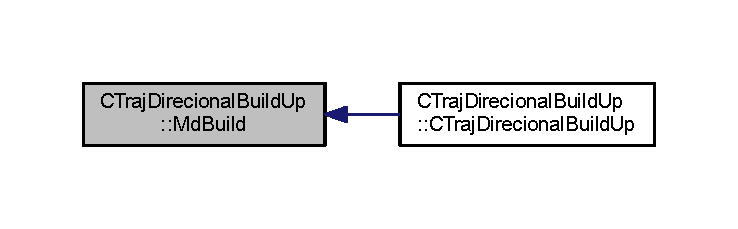
\includegraphics[width=350pt]{class_c_traj_direcional_build_up_a386a6f7a05072e1ed6e8edc310e77a90_icgraph}
\end{center}
\end{figure}
\mbox{\Hypertarget{class_c_traj_direcional_build_up_a8f6f8b3419d26a90601ec7b74c7b137a}\label{class_c_traj_direcional_build_up_a8f6f8b3419d26a90601ec7b74c7b137a}} 
\index{C\+Traj\+Direcional\+Build\+Up@{C\+Traj\+Direcional\+Build\+Up}!Saida\+Dados\+Build@{Saida\+Dados\+Build}}
\index{Saida\+Dados\+Build@{Saida\+Dados\+Build}!C\+Traj\+Direcional\+Build\+Up@{C\+Traj\+Direcional\+Build\+Up}}
\subsubsection{\texorpdfstring{Saida\+Dados\+Build()}{SaidaDadosBuild()}}
{\footnotesize\ttfamily void C\+Traj\+Direcional\+Build\+Up\+::\+Saida\+Dados\+Build (\begin{DoxyParamCaption}{ }\end{DoxyParamCaption})}

E\+X\+I\+BE NO C\+O\+N\+S\+O\+LE OS R\+E\+S\+U\+L\+T\+A\+D\+OS

A\+P�S P\+R\+E\+E\+N\+C\+H\+ER T\+O\+D\+OS OS V\+E\+T\+O\+R\+ES J\+O\+G\+A\+M\+OS NA T\+E\+LA P\+A\+RA C\+O\+N\+F\+E\+R\+IR OS R\+E\+S\+U\+L\+T\+A\+D\+OS Here is the caller graph for this function\+:
\nopagebreak
\begin{figure}[H]
\begin{center}
\leavevmode
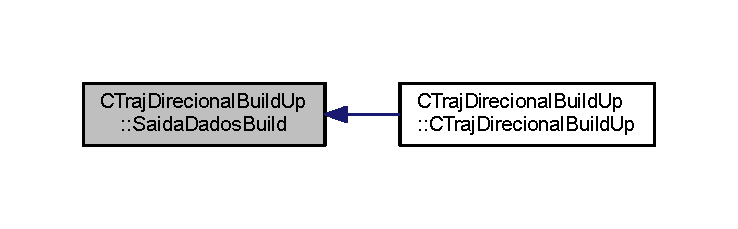
\includegraphics[width=350pt]{class_c_traj_direcional_build_up_a8f6f8b3419d26a90601ec7b74c7b137a_icgraph}
\end{center}
\end{figure}
\mbox{\Hypertarget{class_c_traj_direcional_build_up_a45fb72046a3a4ee60d9ff902a63c866c}\label{class_c_traj_direcional_build_up_a45fb72046a3a4ee60d9ff902a63c866c}} 
\index{C\+Traj\+Direcional\+Build\+Up@{C\+Traj\+Direcional\+Build\+Up}!Tvd\+Build@{Tvd\+Build}}
\index{Tvd\+Build@{Tvd\+Build}!C\+Traj\+Direcional\+Build\+Up@{C\+Traj\+Direcional\+Build\+Up}}
\subsubsection{\texorpdfstring{Tvd\+Build()}{TvdBuild()}}
{\footnotesize\ttfamily void C\+Traj\+Direcional\+Build\+Up\+::\+Tvd\+Build (\begin{DoxyParamCaption}{ }\end{DoxyParamCaption})}

A P\+R\+O\+F\+U\+N\+D\+I\+D\+A\+DE V\+E\+R\+T\+I\+C\+AL � C\+A\+L\+C\+U\+L\+A\+DA U\+T\+I\+L\+I\+Z\+A\+N\+DO O R\+A\+IO DE C\+U\+R\+V\+A\+T\+U\+RA S�O R\+E\+L\+A��\+ES T\+R\+I\+G\+O\+N\+O\+M�\+T\+R\+I\+C\+AS P\+A\+RA E\+N\+C\+O\+N\+T\+R\+AR A P\+A\+R\+TE V\+E\+R\+T\+I\+C\+AL

P\+A\+RA N�O S\+O\+B\+R\+E\+P\+OR V\+A\+L\+O\+R\+ES, I\+N\+I\+C\+I\+A\+M\+OS E\+S\+TE V\+E\+T\+OR 10M D\+E\+P\+O\+IS DO

F\+I\+N\+AL DO V\+E\+T\+OR T\+VD DA P\+A\+R\+TE V\+E\+R\+T\+I\+C\+AL Here is the caller graph for this function\+:
\nopagebreak
\begin{figure}[H]
\begin{center}
\leavevmode
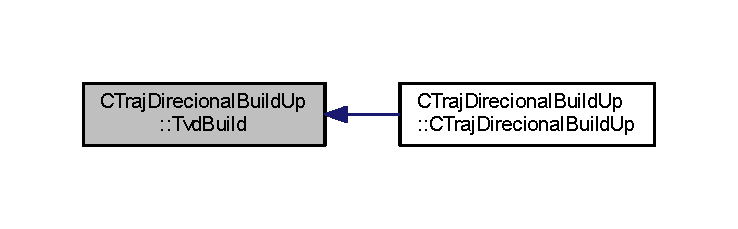
\includegraphics[width=350pt]{class_c_traj_direcional_build_up_a45fb72046a3a4ee60d9ff902a63c866c_icgraph}
\end{center}
\end{figure}


The documentation for this class was generated from the following files\+:\begin{DoxyCompactItemize}
\item 
C\+Traj\+Direcional\+Build\+Up.\+h\item 
C\+Traj\+Direcional\+Build\+Up.\+cpp\end{DoxyCompactItemize}

\hypertarget{class_c_traj_direcional_slant}{}\section{C\+Traj\+Direcional\+Slant Class Reference}
\label{class_c_traj_direcional_slant}\index{C\+Traj\+Direcional\+Slant@{C\+Traj\+Direcional\+Slant}}


Collaboration diagram for C\+Traj\+Direcional\+Slant\+:
\nopagebreak
\begin{figure}[H]
\begin{center}
\leavevmode
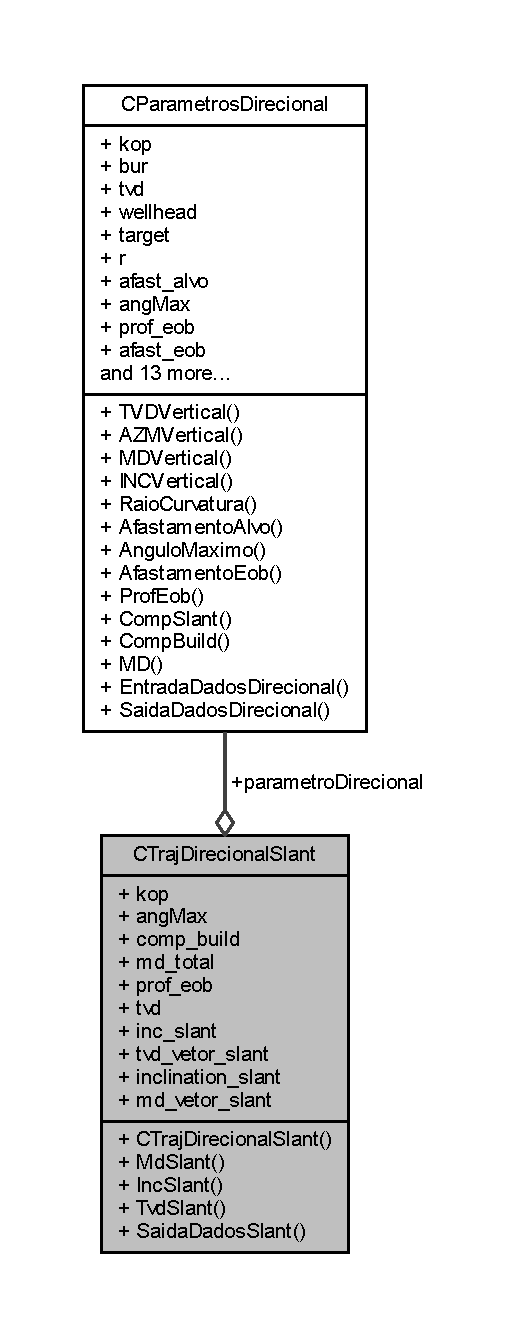
\includegraphics[height=550pt]{class_c_traj_direcional_slant__coll__graph}
\end{center}
\end{figure}
\subsection*{Public Member Functions}
\begin{DoxyCompactItemize}
\item 
\mbox{\Hypertarget{class_c_traj_direcional_slant_a7f87753a8e563e55fbbaf0ebc2fb3829}\label{class_c_traj_direcional_slant_a7f87753a8e563e55fbbaf0ebc2fb3829}} 
\hyperlink{class_c_traj_direcional_slant_a7f87753a8e563e55fbbaf0ebc2fb3829}{C\+Traj\+Direcional\+Slant} (\hyperlink{class_c_parametros_direcional}{C\+Parametros\+Direcional} $\ast$\+\_\+parametro\+Direcional)
\begin{DoxyCompactList}\small\item\em C\+O\+N\+S\+T\+R\+U\+T\+OR R\+E\+C\+E\+B\+E\+N\+DO P\+OR P\+O\+N\+T\+E\+I\+RO AS I\+N\+F\+O\+R\+M\+A��\+ES DA C\+L\+A\+S\+SE \char`\"{}\+C\+P\+A\+R�\+M\+E\+T\+R\+O\+S\+D\+I\+R\+E\+C\+I\+O\+N\+A\+L\char`\"{}. \end{DoxyCompactList}\item 
void \hyperlink{class_c_traj_direcional_slant_a9a9417962ab2b28ac8e509d7806b9c6f}{Md\+Slant} ()
\item 
void \hyperlink{class_c_traj_direcional_slant_a857f2d2c24ccd1f98ff5a97deca30029}{Inc\+Slant} ()
\begin{DoxyCompactList}\small\item\em M�\+T\+O\+D\+OS DA C\+L\+A\+SE. \end{DoxyCompactList}\item 
void \hyperlink{class_c_traj_direcional_slant_adadb99ba28508ad77275d15e745f4663}{Tvd\+Slant} ()
\item 
void \hyperlink{class_c_traj_direcional_slant_a6cd0ccd170ca61a2f7c555720d57a871}{Saida\+Dados\+Slant} ()
\end{DoxyCompactItemize}
\subsection*{Public Attributes}
\begin{DoxyCompactItemize}
\item 
\mbox{\Hypertarget{class_c_traj_direcional_slant_a2e55654073e15e02143c1428c1366e88}\label{class_c_traj_direcional_slant_a2e55654073e15e02143c1428c1366e88}} 
double {\bfseries kop}
\item 
\mbox{\Hypertarget{class_c_traj_direcional_slant_ab29e64ebcca2d43cc2a7997133183b93}\label{class_c_traj_direcional_slant_ab29e64ebcca2d43cc2a7997133183b93}} 
double \hyperlink{class_c_traj_direcional_slant_ab29e64ebcca2d43cc2a7997133183b93}{ang\+Max}
\begin{DoxyCompactList}\small\item\em T\+A\+M\+B�M U\+T\+I\+L\+I\+Z\+A\+M\+OS OS P\+A\+R�\+M\+E\+T\+R\+OS C\+A\+L\+C\+U\+L\+A\+D\+OS NA C\+L\+A\+S\+SE \char`\"{}\+C\+P\+A\+R�\+M\+E\+T\+R\+O\+S\+D\+I\+R\+E\+C\+I\+O\+N\+A\+L\char`\"{}. \end{DoxyCompactList}\item 
\mbox{\Hypertarget{class_c_traj_direcional_slant_a47ec8621913a2ce82da58cde83d89f52}\label{class_c_traj_direcional_slant_a47ec8621913a2ce82da58cde83d89f52}} 
double {\bfseries comp\+\_\+build}
\item 
\mbox{\Hypertarget{class_c_traj_direcional_slant_a50a8df3336fdf96739442c21665bf401}\label{class_c_traj_direcional_slant_a50a8df3336fdf96739442c21665bf401}} 
double {\bfseries md\+\_\+total}
\item 
\mbox{\Hypertarget{class_c_traj_direcional_slant_a6403667a4600ef391d7839717d6138bc}\label{class_c_traj_direcional_slant_a6403667a4600ef391d7839717d6138bc}} 
double {\bfseries prof\+\_\+eob}
\item 
\mbox{\Hypertarget{class_c_traj_direcional_slant_a6ef8234d280f6c1e99a0eb758bac2f46}\label{class_c_traj_direcional_slant_a6ef8234d280f6c1e99a0eb758bac2f46}} 
double {\bfseries tvd}
\item 
\mbox{\Hypertarget{class_c_traj_direcional_slant_ae210b65c6d8bf97e0ee7dc03da7a120e}\label{class_c_traj_direcional_slant_ae210b65c6d8bf97e0ee7dc03da7a120e}} 
double {\bfseries inc\+\_\+slant}
\item 
\mbox{\Hypertarget{class_c_traj_direcional_slant_a05684bbf8f8e6db4cc28d30cf90b338b}\label{class_c_traj_direcional_slant_a05684bbf8f8e6db4cc28d30cf90b338b}} 
std\+::vector$<$ double $>$ {\bfseries tvd\+\_\+vetor\+\_\+slant}
\item 
\mbox{\Hypertarget{class_c_traj_direcional_slant_a705b06d4cf7522c81f2754a3a2d3d217}\label{class_c_traj_direcional_slant_a705b06d4cf7522c81f2754a3a2d3d217}} 
std\+::vector$<$ double $>$ \hyperlink{class_c_traj_direcional_slant_a705b06d4cf7522c81f2754a3a2d3d217}{inclination\+\_\+slant}
\begin{DoxyCompactList}\small\item\em V\+E\+T\+O\+R\+ES Q\+UE S�O C\+R\+I\+A\+D\+OS N\+E\+S\+SA C\+L\+A\+S\+SE. \end{DoxyCompactList}\item 
\mbox{\Hypertarget{class_c_traj_direcional_slant_a30d88d37b15a567d32baaeb92469e44f}\label{class_c_traj_direcional_slant_a30d88d37b15a567d32baaeb92469e44f}} 
std\+::vector$<$ double $>$ {\bfseries md\+\_\+vetor\+\_\+slant}
\item 
\mbox{\Hypertarget{class_c_traj_direcional_slant_afb5d69ee8a6a346bc13e6f1ce50b28a5}\label{class_c_traj_direcional_slant_afb5d69ee8a6a346bc13e6f1ce50b28a5}} 
\hyperlink{class_c_parametros_direcional}{C\+Parametros\+Direcional} $\ast$ {\bfseries parametro\+Direcional}
\end{DoxyCompactItemize}


\subsection{Member Function Documentation}
\mbox{\Hypertarget{class_c_traj_direcional_slant_a857f2d2c24ccd1f98ff5a97deca30029}\label{class_c_traj_direcional_slant_a857f2d2c24ccd1f98ff5a97deca30029}} 
\index{C\+Traj\+Direcional\+Slant@{C\+Traj\+Direcional\+Slant}!Inc\+Slant@{Inc\+Slant}}
\index{Inc\+Slant@{Inc\+Slant}!C\+Traj\+Direcional\+Slant@{C\+Traj\+Direcional\+Slant}}
\subsubsection{\texorpdfstring{Inc\+Slant()}{IncSlant()}}
{\footnotesize\ttfamily void C\+Traj\+Direcional\+Slant\+::\+Inc\+Slant (\begin{DoxyParamCaption}{ }\end{DoxyParamCaption})}



M�\+T\+O\+D\+OS DA C\+L\+A\+SE. 

C\+O\+MO E\+S\+T\+A\+M\+OS NA S\+E��O T\+A\+N\+G\+E\+N\+TE DO P\+O�O, A I\+N\+C\+L\+I\+N\+A��O P\+E\+R\+M\+A\+N\+E\+CE C\+O\+N\+S\+T\+A\+N\+TE

C\+OM O V\+A\+L\+OR DO �\+N\+G\+U\+LO M�\+X\+I\+MO Here is the caller graph for this function\+:
\nopagebreak
\begin{figure}[H]
\begin{center}
\leavevmode
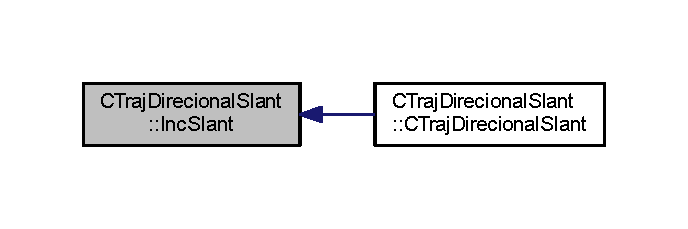
\includegraphics[width=330pt]{class_c_traj_direcional_slant_a857f2d2c24ccd1f98ff5a97deca30029_icgraph}
\end{center}
\end{figure}
\mbox{\Hypertarget{class_c_traj_direcional_slant_a9a9417962ab2b28ac8e509d7806b9c6f}\label{class_c_traj_direcional_slant_a9a9417962ab2b28ac8e509d7806b9c6f}} 
\index{C\+Traj\+Direcional\+Slant@{C\+Traj\+Direcional\+Slant}!Md\+Slant@{Md\+Slant}}
\index{Md\+Slant@{Md\+Slant}!C\+Traj\+Direcional\+Slant@{C\+Traj\+Direcional\+Slant}}
\subsubsection{\texorpdfstring{Md\+Slant()}{MdSlant()}}
{\footnotesize\ttfamily void C\+Traj\+Direcional\+Slant\+::\+Md\+Slant (\begin{DoxyParamCaption}{ }\end{DoxyParamCaption})}

M�\+T\+O\+DO Q\+UE C\+A\+L\+C\+U\+LA O V\+E\+T\+OR DA P\+R\+O\+F\+U\+N\+D\+I\+D\+A\+DE M\+E\+D\+I\+DA P\+A\+RA A S\+E��O T\+A\+N\+G\+E\+N\+TE

A P\+R\+O\+F\+U\+N\+D\+I\+D\+A\+DE M\+E\+D\+I\+DA F\+I\+N\+AL F\+OI C\+A\+L\+C\+U\+L\+A\+DA EM P\+A\+R�\+M\+E\+T\+R\+O\+S\+D\+I\+R\+E\+C\+I\+O\+N\+AL Here is the caller graph for this function\+:
\nopagebreak
\begin{figure}[H]
\begin{center}
\leavevmode
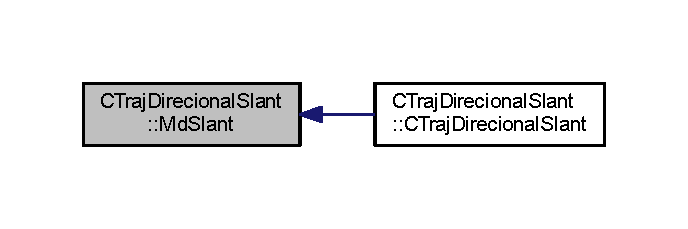
\includegraphics[width=330pt]{class_c_traj_direcional_slant_a9a9417962ab2b28ac8e509d7806b9c6f_icgraph}
\end{center}
\end{figure}
\mbox{\Hypertarget{class_c_traj_direcional_slant_a6cd0ccd170ca61a2f7c555720d57a871}\label{class_c_traj_direcional_slant_a6cd0ccd170ca61a2f7c555720d57a871}} 
\index{C\+Traj\+Direcional\+Slant@{C\+Traj\+Direcional\+Slant}!Saida\+Dados\+Slant@{Saida\+Dados\+Slant}}
\index{Saida\+Dados\+Slant@{Saida\+Dados\+Slant}!C\+Traj\+Direcional\+Slant@{C\+Traj\+Direcional\+Slant}}
\subsubsection{\texorpdfstring{Saida\+Dados\+Slant()}{SaidaDadosSlant()}}
{\footnotesize\ttfamily void C\+Traj\+Direcional\+Slant\+::\+Saida\+Dados\+Slant (\begin{DoxyParamCaption}{ }\end{DoxyParamCaption})}

M�\+T\+O\+DO Q\+UE J\+O\+GA P\+A\+RA A T\+E\+LA T\+O\+D\+OS OS V\+E\+T\+O\+R\+ES C\+A\+L\+C\+U\+L\+A\+D\+OS Here is the caller graph for this function\+:
\nopagebreak
\begin{figure}[H]
\begin{center}
\leavevmode
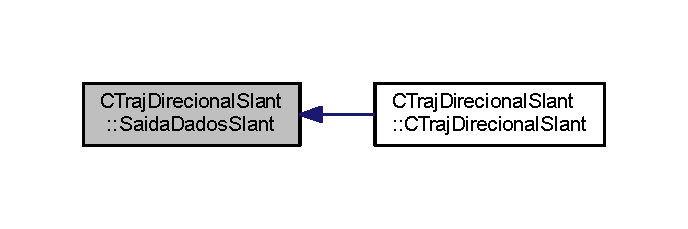
\includegraphics[width=330pt]{class_c_traj_direcional_slant_a6cd0ccd170ca61a2f7c555720d57a871_icgraph}
\end{center}
\end{figure}
\mbox{\Hypertarget{class_c_traj_direcional_slant_adadb99ba28508ad77275d15e745f4663}\label{class_c_traj_direcional_slant_adadb99ba28508ad77275d15e745f4663}} 
\index{C\+Traj\+Direcional\+Slant@{C\+Traj\+Direcional\+Slant}!Tvd\+Slant@{Tvd\+Slant}}
\index{Tvd\+Slant@{Tvd\+Slant}!C\+Traj\+Direcional\+Slant@{C\+Traj\+Direcional\+Slant}}
\subsubsection{\texorpdfstring{Tvd\+Slant()}{TvdSlant()}}
{\footnotesize\ttfamily void C\+Traj\+Direcional\+Slant\+::\+Tvd\+Slant (\begin{DoxyParamCaption}{ }\end{DoxyParamCaption})}

A P\+R\+O\+F\+U\+N\+D\+I\+D\+A\+DE V\+E\+R\+T\+I\+C\+AL F\+I\+N\+AL � C\+A\+L\+C\+U\+L\+A\+DA P\+OR R\+E\+L\+A��\+ES T\+R\+I\+G\+O\+N\+O\+M�\+T\+R\+I\+C\+AS

O V\+A\+L\+OR F\+I\+N\+AL T\+EM Q\+UE B\+A\+T\+ER C\+OM O T\+VD Q\+UE O U\+S\+U�\+R\+IO E\+N\+T\+R\+OU Here is the caller graph for this function\+:
\nopagebreak
\begin{figure}[H]
\begin{center}
\leavevmode
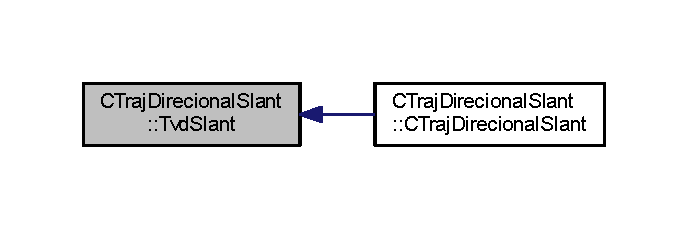
\includegraphics[width=330pt]{class_c_traj_direcional_slant_adadb99ba28508ad77275d15e745f4663_icgraph}
\end{center}
\end{figure}


The documentation for this class was generated from the following files\+:\begin{DoxyCompactItemize}
\item 
C\+Traj\+Direcional\+Slant.\+h\item 
C\+Traj\+Direcional\+Slant.\+cpp\end{DoxyCompactItemize}

\hypertarget{class_c_traj_vertical}{}\section{C\+Traj\+Vertical Class Reference}
\label{class_c_traj_vertical}\index{C\+Traj\+Vertical@{C\+Traj\+Vertical}}


Collaboration diagram for C\+Traj\+Vertical\+:
\nopagebreak
\begin{figure}[H]
\begin{center}
\leavevmode
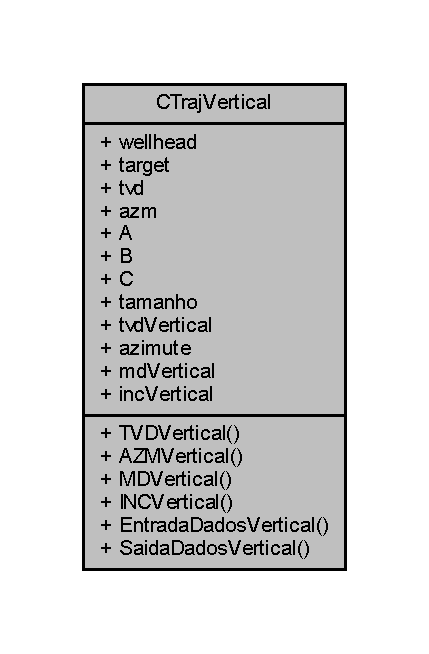
\includegraphics[width=206pt]{class_c_traj_vertical__coll__graph}
\end{center}
\end{figure}
\subsection*{Public Member Functions}
\begin{DoxyCompactItemize}
\item 
void \hyperlink{class_c_traj_vertical_aa42afe0a82f385ba32b6ac041b542213}{T\+V\+D\+Vertical} ()
\begin{DoxyCompactList}\small\item\em Vetor que recebe a inclina��o, constante em 0 na parte vertical. \end{DoxyCompactList}\item 
void \hyperlink{class_c_traj_vertical_af0c9dabb3e989e2f5b54b0eb39d48283}{A\+Z\+M\+Vertical} ()
\begin{DoxyCompactList}\small\item\em M�\+T\+O\+D\+OS DA C\+L\+A\+S\+SE. \end{DoxyCompactList}\item 
void \hyperlink{class_c_traj_vertical_af32e0c76c418bc279425d462cf18e604}{M\+D\+Vertical} ()
\begin{DoxyCompactList}\small\item\em M�\+T\+O\+D\+OS DA C\+L\+A\+S\+SE. \end{DoxyCompactList}\item 
void \hyperlink{class_c_traj_vertical_a1d070eb3b5daa49124c3bed849e0bde0}{I\+N\+C\+Vertical} ()
\begin{DoxyCompactList}\small\item\em M�\+T\+O\+D\+OS DA C\+L\+A\+S\+SE. \end{DoxyCompactList}\item 
void \hyperlink{class_c_traj_vertical_a2e56fe07dd575cb410ce0e3e38220ade}{Entrada\+Dados\+Vertical} ()
\begin{DoxyCompactList}\small\item\em M�\+T\+O\+D\+OS DA C\+L\+A\+S\+SE. \end{DoxyCompactList}\item 
void \hyperlink{class_c_traj_vertical_ae4de85aa1a1e5bc63b160a9b16d80124}{Saida\+Dados\+Vertical} ()
\end{DoxyCompactItemize}
\subsection*{Public Attributes}
\begin{DoxyCompactItemize}
\item 
\mbox{\Hypertarget{class_c_traj_vertical_a06193f45a3eac5e322f5f0444a729a7f}\label{class_c_traj_vertical_a06193f45a3eac5e322f5f0444a729a7f}} 
double {\bfseries wellhead} \mbox{[}2\mbox{]}
\item 
\mbox{\Hypertarget{class_c_traj_vertical_a21d3d8c0f07c5fbb5666d9c1a82d93ec}\label{class_c_traj_vertical_a21d3d8c0f07c5fbb5666d9c1a82d93ec}} 
double \hyperlink{class_c_traj_vertical_a21d3d8c0f07c5fbb5666d9c1a82d93ec}{target} \mbox{[}2\mbox{]}
\begin{DoxyCompactList}\small\item\em D\+A\+D\+OS DE E\+N\+T\+R\+A\+DA DA C\+L\+A\+S\+SE. \end{DoxyCompactList}\item 
\mbox{\Hypertarget{class_c_traj_vertical_af1cd2b66569e1595bfd26a4e3a06fa44}\label{class_c_traj_vertical_af1cd2b66569e1595bfd26a4e3a06fa44}} 
double {\bfseries tvd}
\item 
\mbox{\Hypertarget{class_c_traj_vertical_a8e0f7b2754477302f1ad74dd16f6958e}\label{class_c_traj_vertical_a8e0f7b2754477302f1ad74dd16f6958e}} 
double {\bfseries azm}
\item 
\mbox{\Hypertarget{class_c_traj_vertical_aa50234bb398d53369d48264808755571}\label{class_c_traj_vertical_aa50234bb398d53369d48264808755571}} 
double \hyperlink{class_c_traj_vertical_aa50234bb398d53369d48264808755571}{A}
\begin{DoxyCompactList}\small\item\em P\+A\+R\+A\+M\+E\+T\+R\+OS C\+A\+L\+C\+U\+L\+A\+D\+OS. \end{DoxyCompactList}\item 
\mbox{\Hypertarget{class_c_traj_vertical_ae7caac82a5549ba73a155bef521af4ec}\label{class_c_traj_vertical_ae7caac82a5549ba73a155bef521af4ec}} 
double {\bfseries B}
\item 
\mbox{\Hypertarget{class_c_traj_vertical_a6b874f62d496adb79e45d60d5fe59e02}\label{class_c_traj_vertical_a6b874f62d496adb79e45d60d5fe59e02}} 
double {\bfseries C}
\item 
\mbox{\Hypertarget{class_c_traj_vertical_a138964dc0bc4b06907e3cacafe856b98}\label{class_c_traj_vertical_a138964dc0bc4b06907e3cacafe856b98}} 
int {\bfseries tamanho}
\item 
\mbox{\Hypertarget{class_c_traj_vertical_a727077ea1c053d0675b729cfc484477e}\label{class_c_traj_vertical_a727077ea1c053d0675b729cfc484477e}} 
std\+::vector$<$ double $>$ {\bfseries tvd\+Vertical}
\item 
\mbox{\Hypertarget{class_c_traj_vertical_a7c986198e58acab3759b869238234091}\label{class_c_traj_vertical_a7c986198e58acab3759b869238234091}} 
std\+::vector$<$ double $>$ \hyperlink{class_c_traj_vertical_a7c986198e58acab3759b869238234091}{azimute}
\begin{DoxyCompactList}\small\item\em Vetor que recebe a profundidade vertical, ponto a ponto que ser� calculada. \end{DoxyCompactList}\item 
\mbox{\Hypertarget{class_c_traj_vertical_a6513eb971410f482c6105ef5883258a8}\label{class_c_traj_vertical_a6513eb971410f482c6105ef5883258a8}} 
std\+::vector$<$ double $>$ \hyperlink{class_c_traj_vertical_a6513eb971410f482c6105ef5883258a8}{md\+Vertical}
\begin{DoxyCompactList}\small\item\em Vetor que recebe o azimute, ponto a ponto que ser� calculado. \end{DoxyCompactList}\item 
\mbox{\Hypertarget{class_c_traj_vertical_a0361b36e7b625a554cd300d76f2662a2}\label{class_c_traj_vertical_a0361b36e7b625a554cd300d76f2662a2}} 
std\+::vector$<$ double $>$ \hyperlink{class_c_traj_vertical_a0361b36e7b625a554cd300d76f2662a2}{inc\+Vertical}
\begin{DoxyCompactList}\small\item\em Vetor que recebe a profundidade medida, ponto a ponto que ser� calculada. \end{DoxyCompactList}\end{DoxyCompactItemize}


\subsection{Member Function Documentation}
\mbox{\Hypertarget{class_c_traj_vertical_af0c9dabb3e989e2f5b54b0eb39d48283}\label{class_c_traj_vertical_af0c9dabb3e989e2f5b54b0eb39d48283}} 
\index{C\+Traj\+Vertical@{C\+Traj\+Vertical}!A\+Z\+M\+Vertical@{A\+Z\+M\+Vertical}}
\index{A\+Z\+M\+Vertical@{A\+Z\+M\+Vertical}!C\+Traj\+Vertical@{C\+Traj\+Vertical}}
\subsubsection{\texorpdfstring{A\+Z\+M\+Vertical()}{AZMVertical()}}
{\footnotesize\ttfamily void C\+Traj\+Vertical\+::\+A\+Z\+M\+Vertical (\begin{DoxyParamCaption}{ }\end{DoxyParamCaption})}



M�\+T\+O\+D\+OS DA C\+L\+A\+S\+SE. 

C�\+L\+C\+U\+LO DO P\+A\+R�\+M\+E\+T\+RO A\+Z\+I\+M\+U\+TE DE A\+C\+O\+R\+DO C\+OM A P\+O\+S\+I��O DA S\+O\+N\+DA E DO A\+L\+VO

P\+R\+E\+E\+N\+C\+H\+E\+N\+DO O V\+E\+T\+OR \mbox{\Hypertarget{class_c_traj_vertical_a2e56fe07dd575cb410ce0e3e38220ade}\label{class_c_traj_vertical_a2e56fe07dd575cb410ce0e3e38220ade}} 
\index{C\+Traj\+Vertical@{C\+Traj\+Vertical}!Entrada\+Dados\+Vertical@{Entrada\+Dados\+Vertical}}
\index{Entrada\+Dados\+Vertical@{Entrada\+Dados\+Vertical}!C\+Traj\+Vertical@{C\+Traj\+Vertical}}
\subsubsection{\texorpdfstring{Entrada\+Dados\+Vertical()}{EntradaDadosVertical()}}
{\footnotesize\ttfamily void C\+Traj\+Vertical\+::\+Entrada\+Dados\+Vertical (\begin{DoxyParamCaption}{ }\end{DoxyParamCaption})}



M�\+T\+O\+D\+OS DA C\+L\+A\+S\+SE. 

M�\+T\+O\+DO Q\+UE R\+E\+C\+E\+BE OS D\+A\+D\+OS N\+E\+C\+E\+S\+S�\+R\+I\+OS P\+A\+RA OS C�\+L\+C\+U\+L\+OS DO A\+Z\+I\+M\+U\+TE E T\+VD \mbox{\Hypertarget{class_c_traj_vertical_a1d070eb3b5daa49124c3bed849e0bde0}\label{class_c_traj_vertical_a1d070eb3b5daa49124c3bed849e0bde0}} 
\index{C\+Traj\+Vertical@{C\+Traj\+Vertical}!I\+N\+C\+Vertical@{I\+N\+C\+Vertical}}
\index{I\+N\+C\+Vertical@{I\+N\+C\+Vertical}!C\+Traj\+Vertical@{C\+Traj\+Vertical}}
\subsubsection{\texorpdfstring{I\+N\+C\+Vertical()}{INCVertical()}}
{\footnotesize\ttfamily void C\+Traj\+Vertical\+::\+I\+N\+C\+Vertical (\begin{DoxyParamCaption}{ }\end{DoxyParamCaption})}



M�\+T\+O\+D\+OS DA C\+L\+A\+S\+SE. 

C\+O\+MO O P\+O�O � V\+E\+R\+T\+I\+C\+AL, N�O T\+EM I\+N\+C\+L\+I\+N\+A��O. A\+S\+S\+IM, O V\+E\+T\+OR � P\+R\+E\+E\+N\+C\+H\+I\+DO C\+OM Z\+E\+R\+OS \mbox{\Hypertarget{class_c_traj_vertical_af32e0c76c418bc279425d462cf18e604}\label{class_c_traj_vertical_af32e0c76c418bc279425d462cf18e604}} 
\index{C\+Traj\+Vertical@{C\+Traj\+Vertical}!M\+D\+Vertical@{M\+D\+Vertical}}
\index{M\+D\+Vertical@{M\+D\+Vertical}!C\+Traj\+Vertical@{C\+Traj\+Vertical}}
\subsubsection{\texorpdfstring{M\+D\+Vertical()}{MDVertical()}}
{\footnotesize\ttfamily void C\+Traj\+Vertical\+::\+M\+D\+Vertical (\begin{DoxyParamCaption}{ }\end{DoxyParamCaption})}



M�\+T\+O\+D\+OS DA C\+L\+A\+S\+SE. 

C\+O\+MO O P\+O�O � V\+E\+R\+T\+I\+C\+AL, O MD � I\+G\+U\+AL Q\+UE O T\+VD \mbox{\Hypertarget{class_c_traj_vertical_ae4de85aa1a1e5bc63b160a9b16d80124}\label{class_c_traj_vertical_ae4de85aa1a1e5bc63b160a9b16d80124}} 
\index{C\+Traj\+Vertical@{C\+Traj\+Vertical}!Saida\+Dados\+Vertical@{Saida\+Dados\+Vertical}}
\index{Saida\+Dados\+Vertical@{Saida\+Dados\+Vertical}!C\+Traj\+Vertical@{C\+Traj\+Vertical}}
\subsubsection{\texorpdfstring{Saida\+Dados\+Vertical()}{SaidaDadosVertical()}}
{\footnotesize\ttfamily void C\+Traj\+Vertical\+::\+Saida\+Dados\+Vertical (\begin{DoxyParamCaption}{ }\end{DoxyParamCaption})}

C\+H\+A\+M\+A\+N\+DO T\+O\+D\+OS OS M�\+T\+O\+D\+OS

C\+O\+N\+F\+I\+G\+U\+R\+A\+N\+DO A S\+A�\+DA E F\+A\+Z\+E\+N\+DO O C\+A\+B\+E�\+A\+L\+HO

G\+E\+R\+A\+N\+DO A S\+A�\+DA DE U\+MA F\+O\+R\+MA O\+R\+G\+A\+N\+I\+Z\+A\+DA

P\+R\+E\+C\+I\+S�O DE D\+U\+AS C\+A\+S\+AS D\+E\+C\+I\+M\+A\+IS

A\+L\+I\+N\+H\+A\+M\+E\+N\+TO A D\+I\+R\+E\+I\+TA C\+OM T\+A\+B\+U\+L\+A��O

A\+R\+Q\+U\+I\+VO C\+OM A T\+A\+B\+E\+LA D\+OS R\+E\+S\+U\+L\+T\+A\+D\+OS F\+I\+N\+A\+IS DO P\+R\+O\+G\+R\+A\+MA \mbox{\Hypertarget{class_c_traj_vertical_aa42afe0a82f385ba32b6ac041b542213}\label{class_c_traj_vertical_aa42afe0a82f385ba32b6ac041b542213}} 
\index{C\+Traj\+Vertical@{C\+Traj\+Vertical}!T\+V\+D\+Vertical@{T\+V\+D\+Vertical}}
\index{T\+V\+D\+Vertical@{T\+V\+D\+Vertical}!C\+Traj\+Vertical@{C\+Traj\+Vertical}}
\subsubsection{\texorpdfstring{T\+V\+D\+Vertical()}{TVDVertical()}}
{\footnotesize\ttfamily void C\+Traj\+Vertical\+::\+T\+V\+D\+Vertical (\begin{DoxyParamCaption}{ }\end{DoxyParamCaption})}



Vetor que recebe a inclina��o, constante em 0 na parte vertical. 

L�\+G\+I\+CA P\+A\+RA E\+V\+I\+T\+AR P\+A\+S\+SO DE T\+E\+M\+PO S\+EM S\+ER I\+N\+T\+E\+I\+RO

C\+R\+I\+A��O DO V\+E\+T\+OR T\+VD, D\+I\+V\+I\+D\+I\+N\+DO O T\+VD T\+O\+T\+AL, P\+E\+LO E\+S\+P\+A�O EM (m) Q\+UE Q\+U\+E\+R\+E\+M\+OS 

The documentation for this class was generated from the following files\+:\begin{DoxyCompactItemize}
\item 
C\+Traj\+Vertical.\+h\item 
C\+Traj\+Vertical.\+cpp\end{DoxyCompactItemize}

%--- End generated contents ---

% Index
\backmatter
\newpage
\phantomsection
\clearemptydoublepage
\addcontentsline{toc}{chapter}{Index}
\printindex

\end{document}
